\documentclass[11pt]{article}
\usepackage{fullpage}
\usepackage{amsmath, amsfonts}
\usepackage[utf8]{inputenc}
\usepackage{float}
\usepackage{tikz}
\usepackage{graphicx}
\usepackage{booktabs}
\usepackage{listings}
\usepackage{todonotes}
\usepackage{multirow}
\usepackage{verbatim}

\usepackage{hyperref}
%\hypersetup{
%    colorlinks=true,
%    linkcolor=blue,
%    filecolor=magenta,      
%    urlcolor=cyan,
%}

\usepackage[toc,page]{appendix}
\renewcommand{\lstlistingname}{Algorithm}% Listing -> Algorithm
\renewcommand{\lstlistlistingname}{List of \lstlistingname s}% List of Listings -> List of Algorithms
% \lstlistoflistings
\definecolor{mGreen}{rgb}{0,0.6,0}
\definecolor{mGray}{rgb}{0.5,0.5,0.5}
\definecolor{mPurple}{rgb}{0.58,0,0.82}
\definecolor{backgroundColour}{rgb}{0.95,0.95,0.92}

\lstdefinestyle{CStyle}{
    backgroundcolor=\color{backgroundColour},   
    basicstyle=\footnotesize\ttfamily,
    keywordstyle=\bfseries\color{green!40!black},
    commentstyle=\itshape\color{purple!40!black},
    identifierstyle=\color{blue},
    stringstyle=\color{orange},
    breakatwhitespace=false,         
    breaklines=true,                 
    captionpos=b,                    
    keepspaces=true,                 
    numbers=left,                    
    numbersep=5pt,                  
    showspaces=false,                
    showstringspaces=false,
    showtabs=false,                  
    tabsize=4,
    language=C
}

\lstdefinestyle{customc}{
  belowcaptionskip=1\baselineskip,
  breaklines=true,
  frame=L,
  xleftmargin=\parindent,
  language=C,
  showstringspaces=false,
  basicstyle=\footnotesize\ttfamily,
  keywordstyle=\bfseries\color{green!40!black},
  commentstyle=\itshape\color{purple!40!black},
  identifierstyle=\color{blue},
  stringstyle=\color{orange},
}


\usepackage{url}

%%%%%%% Litterature list %%%%%%%
\usepackage[%
 backend=bibtex      % biber or bibtex
%,style=authoryear    % Alphabeticalsch
 ,style=numeric  % numerical-compressed
 ,sorting=none        % no sorting
 ,sortcites=true      % some other example options ...
 ,block=none
 ,indexing=false
 ,citereset=none
 ,isbn=true
 ,url=true
 ,doi=true            % prints doi
 ,natbib=true         % if you need natbib functions
]{biblatex}
\addbibresource{contents/refs.bib}  % better than \bibliography
\usepackage{caption}
\usepackage{subcaption}
\usepackage{pgfplots}
\usepackage{tikz}
\usetikzlibrary{arrows, positioning, calc}

\newcommand*{\Ph}{\hphantom{{}+{}}}%


\begin{document}
\begin{center}
{{\Large \sc High-Performance Computing}}
\end{center}
\rule{\textwidth}{1pt}
\begin{description}
\item[Student name and id:] Marie Mørk \{s112770\} Anja Liljedahl Christensen\{s162876\}
 Andreas Vedel Jantzen \{s162858\}
 Anders Launer Bæk \{s160159\}
\item[Hold name:] matmult\_MAAA
\item[Hand-in:] Matrix Multiplication
\end{description}
\rule{\textwidth}{1pt}


\section{Summary}
Different functions, performing matrix-matrix multiplication are implemented in C in order to compare performance. Cases considered are ordering of the nested loops, optimizers in the compiler and blocking. The implemented functions are compared with the CBLAS subroutine DGEMM. As memory in C is stored row-wise, it has been found that the most optimal ordering of nested loops is to have the column index in the most inner loop. The optimizers are found to enhance performance significantly. The blocked version is found to be less efficient than the optimized version of the most efficient ordering of the loops. This might be due to the implementation of the blocking in which as many columns as rows are considered at a time. 

\section{Statement of the problem}

The goal of the assignment is to create a library of functions that perform matrix-matrix multiplications. Performance of the implementations are to be compared with the DGEMM matrix-matrix multiplication routine from the BLAS library. As input, each of the functions should take the dimensions of the matrices (M, N, K) as well as the matrices (A, B, C), according to figure \ref{fig:matmult}. The problem is divided into four sub-problems; 
\begin{itemize}
    \item Wrap the call DGEMM into a function called \texttt{matmult\_lib()}, that takes the same inputs as
    specified above.
    \item Implement a function that performs double precision matrix-matrix multiplication. The function should be named \texttt{matmult\_nat()}.
    \item Functions for each of the permutations of the three nested loops needed to perform matrix multiplications. The performance of the permutations should be compared. Furthermore, the timings should be compared with and without different compiler optimizations. The functions should be named as \texttt{matmult\_per()}, where \texttt{per} is the ordering of the nested loops for the given implementation, e.g. \texttt{nmk,knm}, ect.
    \item A blocked version of the matrix-matrix multiplication function named \texttt{matmult\_blk()}. This function should take an extra input, \texttt{bs}, which specifies the blocking size.
\end{itemize}

\begin{figure}[h]
    \centering
    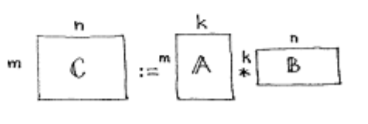
\includegraphics[]{contents/pics_1/matmult.PNG}
    \caption{Visualisation of the matrix-matrix multiplications to be performed. The picture is taken from the problem description on DTU Inside.}
    \label{fig:matmult}
\end{figure}

\section{Hardware and software}\label{sec:hard}

Specifications of the test environment are listed below:
\begin{itemize}
\item CPU information
\begin{itemize}
\item Vendor ID:             GenuineIntel
\item CPU family:            6
\item Model:                 79
\item Model name:            Intel(R) Xeon(R) CPU E5-2650 v4 @ 2.20GHz
\item CPU MHz:               1297.656
\item L1 (d / i) cache:             32K
\item L2 cache:              256K
\item L3 cache:              30720K
\end{itemize}
\item Compiler and Matrix implementations
\begin{itemize}
\item The GCC compiler have been applied with and without compiler optimization using the compiler flag \texttt{-Ofast}. 
\item The library function uses DGEMM from the CBLAS interface
\item Matrices are indexed in the following way: [m] [n]
\item The following line has been specified in the job script: "\texttt{\#BSUB -n 1}" to make sure the batch job only uses one core.
\end{itemize}
\end{itemize}


\section{Theory}
Matrix multiplications are central operations in many numerical algorithms. Due to this, it is essential to make the operation fast to keep the computation time low. In order to achieve an optimal matrix-matrix multiplication algorithm, it is therefore important to take the ordering of nested loops and memory storage in the computer into account.\\


In C matrices are stored row-wise. Hence, when an element is fetched from memory the next couple of elements in the same row are collected as well, since they are stored in the same cache line. This is useful if the next couple of elements from the same row are needed in the near future, since they have already been loaded into memory. If on the other hand the next element is extracted from another row, e.g. in the case of looping through a column, there will be a cache miss and a new cache line is loaded into memory. Thus, in the worst case there will be a cache miss each time a new element is needed. In the case of matrix multiplication it is necessary to loop through both rows and columns in multiple nested loops and hence there is a great chance of cache miss when the matrices are sufficiently large. If the matrices are small enough such that all three will fit in memory there should be no cache misses. For large scale matrices it is essential to optimize the implementation of the matrix-matrix multiplication in order to avoid too many cache misses.\\

Double precision matrix multiplication of square matrices requires space for $3\cdot d^3$ doubles in memory, if the dimensions of the matrices is given by $d$. As storage of a double takes up 8 bits, the maximum dimensions for the matrices to fit in the memory of a given cache is found theoretically by calculating
\begin{align*}
    d = \sqrt{\frac{L/8}{3}}
\end{align*}
where L is the memory in the given cache. The maximum dimensions of square matrices fitting into each of the caches used are listed in table \ref{tab:cache_max_dim}. In reality, the maximum allowed dimensions might be higher, as the program performs hardware prefetch. 
\begin{table}[h]
    \centering
    \begin{tabular}{c|c|c}
         Cache & Size [bytes] & Maximum dimension of Matrix  \\ \hline
         $L_1$ & 32K & 36 \\
         $L_2$ & 256K & 103 \\
         $L_3$ & 30720K & 1131 
    \end{tabular}
    \caption{Maximum dimensions of square matrices fitting into each of the caches.}
    \label{tab:cache_max_dim}
\end{table}

In the last sub problem of the report, blocking is implemented in order to optimize the memory usage in the algorithm. The idea behind blocking is to divide the iterations into smaller blocks, so that operations can be performed for parts of the matrices at a time, instead of considering the full size of the problem. This is especially useful when handling large problems, for which the memory needed to compute the full operation exceeds the bounds of the memory. When using an algorithm that relies on blocking it is important to use one of the respective compiler flags: \texttt{-O3} or \texttt{-Ofast}. By doing so the compiler analyses the code several lines ahead and is hereby able to optimize the code. 
%Notet med optimizers i compileren

%Noget med blocking (evt. sammen med hukommelse) 

% hardware prefetch

%Hit/miss og mflops/s - memory 

\section{Algorithms}
\subsection{\texttt{matmult\_lib}} %Wrapping of GDEMM
The subroutine DGEMM from the library BLAS will be used to evaluate the performance of and compare with the different implementations of the matrix-matrix multiplication. For this purpose the CBLAS interface is used and wrapped into the function \texttt{matmult\_lib} such that the library implementation of the matrix-matrix multiplication takes the same arguments as the other functions.  The call to DGEMM using the CBLAS interface is \texttt{cblas\_dgemm} which takes 14 arguments\footnote{http://www.netlib.org/lapack/explore-html/dc/d18/cblas} as shown in algorithm \ref{alg:lib}. From the inputs, the matrix multiplication is calculated as
\begin{align*}
    C = \alpha \cdot A \cdot B + \beta \cdot C.
\end{align*}
Here, $\alpha$ and $\beta$ are arguments to be specified in the input. In this case $\alpha$ is set to 1 while $\beta$ is set to 0 in order to get the wanted output. The other inputs in DGEMM (aside from M, N, K, A, B, and C) are the layout (set to rowmajor), whether the A and B matrices should be transposed (TRANSA and TRANSB) and the leading dimensions of A, B and C. As seen in the algorithm \ref{alg:lib}, the A and B matrices are not transposed, and the dimensions are set to K, N and N for A, B and C. 
\lstinputlisting[label={alg:lib},caption={\texttt{matmult\_lib}},style=CStyle]{code/matmult_lib.c}

\subsection{\texttt{matmult\_nat}} %nat
The implementation of the \texttt{matmult\_nat} function is listed in algorithm \ref{alg:nat}. For this function, it has been chosen to use the a MNK ordering of the nested loops. That is that the outer loop iterates over the dimension M, the second over N and the inner over K. 
\lstinputlisting[label={alg:nat},caption={\texttt{matmult\_nat}},style=CStyle]{code/matmult_nat.c}

\subsection{\texttt{matmult\_per}} % permutations
The \texttt{matmult\_per} permutations are implemented as presented in algorithm \ref{alg:per}, where the ordering of the nested loops are interchanged for each permutation of M, N and K. There exist six different permutations of the \texttt{matmult\_nat} function, namely MNK, NKM, MKN, KMN, MNK, and NMK. The \texttt{matmult\_per} algorithm has been optimized in relation to the \texttt{matmult\_nat} function. This has been done using stripmining, and setting all entries of C to zero using 1 for loop instead of 2 enables the compiler to perform vectorization.
\lstinputlisting[label={alg:per},caption={\texttt{matmult\_per} for the \texttt{mnk} ordering of the loops.},style=CStyle]{code/permutationcodepiece.c}

\subsection{\texttt{matmult\_blk}} % Blocking
In order to implement blocking in the matrix-matrix multiplications, additional nested loops are needed. The algorithm used for blocking is based on one of the best performing versions of the \texttt{matmult\_per} functions – in this case \texttt{matmult\_mkn}. In algorithm \ref{alg:blk} the function is presented. As mentioned in the problem description \texttt{matmult\_blk} takes the additional input \texttt{bs}, which is the blocking size. In blocking, the matrices A, B and C are portioned into smaller matrices for which the multiplications are performed and then added to each other to get the full C matrix. In this implementation the blocks are chosen to be square matrices. This can be seen from the first three nested loops in which blocks of the matrices of size bs$\times$bs are chosen. In the inner three nested loops the extracted matrices are multiplied and added to C. When using \texttt{matmult\_blk} the compiler needs an optimizer flag, in order for the blocking to set in. 
\lstinputlisting[label={alg:blk},caption={\texttt{matmult\_blk}},style=CStyle]{code/matmult_blk.c}





\newpage
\section{Results}
The implementation of the different functions were checked in a test-script to see if the C matrix was calculated as expected. Each of the functions \texttt{matmult\_nat}, \texttt{matmult\_per}, \texttt{matmult\_blk}, and \texttt{matmult\_lib} were tested using the square matrices:
\begin{align*}
    A_s = 
    \begin{pmatrix}
        1 & 2\\
        2 & 4
    \end{pmatrix} \qquad
    B_s =
    \begin{pmatrix}
        2 & 2\\
        2 & 2
    \end{pmatrix}
\end{align*}
and the non-square matrices:
\begin{align*}
    A_{ns} = 
    \begin{pmatrix}
        1 & 2\\
        2 & 4\\
        3 & 6
    \end{pmatrix} \qquad
    B_{ns} =
    \begin{pmatrix}
        2 & 2 & 2\\
        2 & 2 & 2
    \end{pmatrix}
\end{align*}
which all returned
\begin{align*}
    C_{s} = 
    \begin{pmatrix}
        6 & 6\\
        12 & 12
    \end{pmatrix} \qquad
    C_{ns} = 
    \begin{pmatrix}
        6 & 6 & 6\\
        12 & 12 & 12\\
        18 & 18 & 18
    \end{pmatrix}
\end{align*}
% The calculations are checked against the DGEMM subroutine to ensure that the matrix-matrix multiplication is computed correctly for each of the implemented functions. 
The calculation check sum provided by the driver has also been studied during the performance evaluation of the implemented functions, and in each of the cases the return value was 0 as expected.  

Only square matrices are considered, e.g. N = M = K when the performance of the functions is evaluated. 

Furthermore the performances of the above functions have been evaluated with and without the compiler flag \texttt{-Ofast} which enable compiler optimization, indicated as "opt".
It has been decided to capture the hit and miss counters for the L1 cache and L2 cache in the first project.

\subsection{Performance of \texttt{matmult\_nat}}

Figure \ref{fig:nat_perf} illustrates two realizations of the naive implementation of the \texttt{matmult\_nat} function. The blue realization is the naive implementation without compiler optimization enabled and the black realization has compiler optimization enabled. By considering the differences between the realizations in figure \ref{fig:nat_perf} huge increases in performance can be achieved by using compiler optimization.\\

\begin{figure}[!th]
\centering
\begin{tikzpicture}[scale = 1]
\begin{axis}[
width=17cm, height=8cm,     % size of the image
grid = major,
grid style={dashed, gray!30},
xmode=log,log basis x=10,
xmin=0,    % start the diagram at this
ymin=50,    % start the diagram at this 
ymax=2000, % end   the diagram at this 
axis background/.style={fill=white},
ylabel=Mflops/s,
xlabel=Memory/kbytes]

\addplot[mark=*, blue] table [x=mem, y=mflops, col sep=comma]{data/matmult_nat.txt};
\addlegendentry{matmult\_nat}
\addplot[mark=*, black] table [x=mem, y=mflops, col sep=comma]{data/matmult_nat_opt.txt};
\addlegendentry{matmult\_nat\_opt}


\addplot[red] table [x=x, y=y, col sep=comma]{data/L1.txt};
\addplot[red] table [x=x, y=y, col sep=comma]{data/L2.txt};
\addplot[red] table [x=x, y=y, col sep=comma]{data/L3.txt};
\addlegendentry{L1, L2 and L3 cache}
\end{axis} 
\end{tikzpicture}
\caption{Performance of the \texttt{matmult\_nat} function measured in Mflops/s as a function of kbytes.}
\label{fig:nat_perf}
\end{figure}


Table \ref{tab:L1L2hitmis_nat} reports the cache hits and cache miss for the \texttt{matmult\_nat} function. It is observed that there are fewer hits in the optimized version for the L1 cache, while the misses are of equal size. The hypothesis would be that the number of hits increases for the optimized version, but it might be that the optimizer reduces the memory to be fetched, why the number of hits drops. Even though the number of hits reduces, we can still conclude that the optimized function performs significantly better than the non-optimized.

\begin{table}[!th]
\centering
\begin{tabular}{l|rr|rr|rr|rr}
\multirow{3}{*}{} & \multicolumn{4}{|c}{Non-optimized}& \multicolumn{4}{|c}{Optimized}\\
& \multicolumn{2}{|c}{L1 in $\%$} & \multicolumn{2}{|c}{L2 in $\%$}& \multicolumn{2}{|c}{L1 in $\%$} & \multicolumn{2}{|c}{L2 in $\%$} \\
& Hit& Miss& Hit& Miss& Hit& Miss& Hit& Miss\\ \hline
\texttt{matmult\_nat(50x50)}& 10 & 0 & 0 & 0 &0 & 0 & 0 & 0\\
\texttt{matmult\_nat(850x850)} & 129129 & 6072 & 5368 & 704 & 11651 & 6069 & 5524 & 544\\
\texttt{matmult\_nat(1600x1600)}& 861503 & 34583 & 134 & 34445& 73553 & 31510 & 92 & 31416\\
\end{tabular}
\caption{Hits and miss of the L1 and L2 cache for nat, presented in millions}
\label{tab:L1L2hitmis_nat}
\end{table}
\newpage

The naive implementation of the matrix multiplication routine, \texttt{matmult\_nat} is compared to the library subroutine DGEMM, which has been wrapped in \texttt{matmult\lib}. In figure \ref{fig:nat_perf}, the performance of DGEMM is shown with and without optimization in the compiler. Please note, that the axes is different from the one in \ref{fig:nat_perf}.\\
It is seen from the figure that the performance of DGEMM is nearly the same whether or not an optimizer is used in the compiler. This is not surprising, as we expect the library function to be optimized in itself, and the wrapper funciton \texttt{matmult\_lib} only calls the DGEMM subroutine and assigns values to some of the inputs. The performance of the library sub routine is significantly better than that of \texttt{matmult\_nat}. In table \ref{tab:L1L2hitmis_lib}, the hits and miss of the function are shown. All hits and misses are seen to be zero. This might be a consequence of the way the analyzer function handles the wrapper function. We would have expected the library function to have a very high number of hits and only few misses.

\begin{figure}[!th]
\centering
\begin{tikzpicture}[scale = 1]
\begin{axis}[
width=17cm, height=8cm,     % size of the image
grid = major,
grid style={dashed, gray!30},
xmode=log,log basis x=10,
%xmin=0,    % start the diagram at this
%ymin=50,    % start the diagram at this 
ymax=10000, % end   the diagram at this 
axis background/.style={fill=white},
ylabel=Mflops/s,
xlabel=Memory/kbytes,
legend pos=south east]

%\addplot[mark=*, blue] table [x=mem, y=mflops, col sep=comma]{data/matmult_nat.txt};
%\addlegendentry{matmult\_nat}
\addplot[mark=*, black] table [x=mem, y=mflops, col sep=comma]{data/matmult_lib_opt.txt};
\addlegendentry{matmult\_lib\_opt}

\addplot[mark=*, blue] table [x=mem, y=mflops, col sep=comma]{data/matmult_lib.txt};
\addlegendentry{matmult\_lib}


\addplot[red] table [x=x, y=y, col sep=comma]{data/L1.txt};
\addplot[red] table [x=x, y=y, col sep=comma]{data/L2.txt};
\addplot[red] table [x=x, y=y, col sep=comma]{data/L3.txt};
\addlegendentry{L1, L2 and L3 cache}
\end{axis} 
\end{tikzpicture}
\caption{Performance of the \texttt{matmult\_lib} function measured in Mflops/s as a function of kbytes.}
\label{fig:nat_perf}
\end{figure}

\begin{table}[!th]
\centering
\begin{tabular}{l|rr|rr|rr|rr}
\multirow{3}{*}{} & \multicolumn{4}{|c}{Non-optimized}& \multicolumn{4}{|c}{Optimized}\\
& \multicolumn{2}{|c}{L1 in $\%$} & \multicolumn{2}{|c}{L2 in $\%$}& \multicolumn{2}{|c}{L1 in $\%$} & \multicolumn{2}{|c}{L2 in $\%$} \\
& Hit& Miss& Hit& Miss& Hit& Miss& Hit& Miss\\ \hline
\texttt{matmult\_lib(50x50)}& 0.0 & 0.0 & 0.0 & 0.0&0.0 & 0.0 & 0.0 & 0.0\\
\texttt{matmult\_lib(850x850)}& 0.0 & 0.0 & 0.0 & 0.0 & 0.0 & 0.0 & 0.0 & 0.0\\
\texttt{matmult\_lib(1600x1600)}& 0.0 & 0.0 & 0.0 & 0.0& 0.0 & 0.0 & 0.0 & 0.0\\
\end{tabular}
\caption{Hits and miss of the L1 and L2 cache for lib, presented in millions}
\label{tab:L1L2hitmis_lib}
\end{table}


\newpage
\subsection{Optimal permutations of \texttt{matmult\_nat}}

As mentioned earlier it is possible to create several permutations of the naive \texttt{matmult\_nat} function. The six possible (the naive is included) permutations are presented in figure \ref{fig:opt_nmk_1_non} and the compiler optimized permutations in figure \ref{fig:opt_nmk_1}.


\begin{figure}[!th]
\centering
\begin{tikzpicture}[scale = 1]
\begin{axis}[
width=17cm, height=8cm,     % size of the image
grid = major,
grid style={dashed, gray!30},
xmode=log,log basis x=10,
xmin=0,    % start the diagram at this
ymin=50,    % start the diagram at this 
ymax=400, % end   the diagram at this 
axis background/.style={fill=white},
ylabel=Mflops/s,
xlabel=Memory/kbytes,
legend pos=south west]

\addplot[mark=*, black] table [x=mem, y=mflops, col sep=comma]{data/matmult_nmk.txt};
\addlegendentry{nmk}

\addplot[mark=*, red] table [x=mem, y=mflops, col sep=comma]{data/matmult_nkm.txt};
\addlegendentry{nkm}

\addplot[mark=*, blue] table [x=mem, y=mflops, col sep=comma]{data/matmult_mnk.txt};
\addlegendentry{mnk}



\addplot[mark=*, orange] table [x=mem, y=mflops, col sep=comma]{data/matmult_mkn.txt};
\addlegendentry{mkn}

\addplot[mark=*, green] table [x=mem, y=mflops, col sep=comma]{data/matmult_knm.txt};
\addlegendentry{knm}

\addplot[mark=*, magenta] table [x=mem, y=mflops, col sep=comma]{data/matmult_kmn.txt};
\addlegendentry{kmn}

\addplot[red] table [x=x, y=y, col sep=comma]{data/L1.txt};
\addplot[red] table [x=x, y=y, col sep=comma]{data/L2.txt};
\addplot[red] table [x=x, y=y, col sep=comma]{data/L3.txt};
%\addlegendentry{L1, L2 and L3 cache}
\end{axis} 
\end{tikzpicture}
\caption{Performance of all permutations of the \texttt{matmult\_per} functions measured in Mflops/s as a function of kbytes.}
\label{fig:opt_nmk_1_non}
\end{figure}

\begin{figure}[!th]
\centering
\begin{tikzpicture}[scale = 1]
\begin{axis}[
width=17cm, height=8cm,     % size of the image
grid = major,
grid style={dashed, gray!30},
xmode=log,log basis x=10,
xmin=0,    % start the diagram at this
ymin=0,    % start the diagram at this 
ymax=5000, % end   the diagram at this 
axis background/.style={fill=white},
ylabel=Mflops/s,
xlabel=Memory/kbytes,
legend pos=north west]

\addplot[mark=*, black] table [x=mem, y=mflops, col sep=comma]{data/matmult_nmk_opt.txt};
\addlegendentry{nmk\_opt}

\addplot[mark=*, red] table [x=mem, y=mflops, col sep=comma]{data/matmult_nkm_opt.txt};
\addlegendentry{nkm\_opt}

\addplot[mark=*, blue] table [x=mem, y=mflops, col sep=comma]{data/matmult_mnk_opt.txt};
\addlegendentry{mnk\_opt}



\addplot[mark=*, orange] table [x=mem, y=mflops, col sep=comma]{data/matmult_mkn_opt.txt};
\addlegendentry{mkn\_opt}

\addplot[mark=*, green] table [x=mem, y=mflops, col sep=comma]{data/matmult_knm_opt.txt};
\addlegendentry{knm\_opt}

\addplot[mark=*, magenta] table [x=mem, y=mflops, col sep=comma]{data/matmult_kmn_opt.txt};
\addlegendentry{kmn\_opt}

\addplot[red] table [x=x, y=y, col sep=comma]{data/L1.txt};
\addplot[red] table [x=x, y=y, col sep=comma]{data/L2.txt};
\addplot[red] table [x=x, y=y, col sep=comma]{data/L3.txt};
%\addlegendentry{L1, L2 and L3 cache}
\end{axis} 
\end{tikzpicture}
\caption{Performance of all permutations of the the compiler optimized \texttt{matmult\_***} functions measured in Mflops/s as a function of kbytes.}
\label{fig:opt_nmk_1}
\end{figure}

% \begin{figure}[!th]
% \centering
% \begin{tikzpicture}[scale = 1]
% \begin{axis}[
% width=17cm, height=8cm,     % size of the image
% grid = major,
% grid style={dashed, gray!30},
% xmode=log,log basis x=10,
% xmin=0,    % start the diagram at this
% ymin=0,    % start the diagram at this 
% ymax=5000, % end   the diagram at this 
% axis background/.style={fill=white},
% ylabel=Mflops/s,
% xlabel=Memory/kbytes,
% legend pos=north west]

% \addplot[mark=*, black] table [x=mem, y=mflops, col sep=comma]{data/matmult_mkn_opt.txt};
% \addlegendentry{mkn\_opt}

% \addplot[mark=*, red] table [x=mem, y=mflops, col sep=comma]{data/matmult_knm_opt.txt};
% \addlegendentry{knm\_opt}

% \addplot[mark=*, blue] table [x=mem, y=mflops, col sep=comma]{data/matmult_kmn_opt.txt};
% \addlegendentry{kmn\_opt}

% \addplot[red] table [x=x, y=y, col sep=comma]{data/L1.txt};
% \addplot[red] table [x=x, y=y, col sep=comma]{data/L2.txt};
% \addplot[red] table [x=x, y=y, col sep=comma]{data/L3.txt};
% %\addlegendentry{L1, L2 and L3 cache}
% \end{axis} 
% \end{tikzpicture}
% \caption{Performance of the compiler optimized \texttt{matmult\_mkn}, \texttt{matmult\_knm} and \texttt{matmult\_kmn} functions measured in Mflops/s as a function of kbytes.}
% \label{fig:opt_nmk_2}
% \end{figure}

Figure \ref{fig:opt_nmk_1_non} tells that \texttt{matmult\_mkn} and \texttt{matmult\_kmn} are the best performing permutations in the L3 cache. Hence having N as the last index, makes the matrix-matrix multiplication the fastest. This was also expected, because M and K are the row indexes of the input matrices and fits to the way memory is stored the most efficient way. \\
The permutations has calculated using an optimizer. This result is presented in \ref{fig:opt_nmk_1}. This confirms that \texttt{matmult\_mkn} and \texttt{matmult\_kmn} are the fastest permutations, having \texttt{matmult\_mkn} a bit faster. When the optimizer is used the performance difference already occours in L1 and definately in L2. Hence, the combination of optimizer and having the right indexing makes \texttt{matmult\_mkn} the fastest permutation. \\ 
Table \ref{tab:L1L2hitmis_1600}, \ref{tab:L1L2hitmis_850} and \ref{tab:L1L2hitmis_50} presents the cache hits and misses for L1 and L2.
The functions have been evaluated for 50, 850 and 1600 and the global variable \texttt{} has been set to perform 10 iterations in each loop in order to make comparable tests. Table \ref{tab:L1L2hitmis_850} and \ref{tab:L1L2hitmis_1600} does again confirm that \texttt{matmult\_mkn} and \texttt{matmult\_kmn} are the most optimal matrix-matrix multiplication indexing. This can be concluded because the ratio of their respective hits and misses are big, both for L1 and L2. 

\begin{table}[!th]
\centering
\begin{tabular}{l|rr|rr|rr|rr}
\multirow{3}{*}{50x50} & \multicolumn{4}{|c}{Non-optimized}& \multicolumn{4}{|c}{Optimized}\\
& \multicolumn{2}{|c}{L1} & \multicolumn{2}{|c}{L2}& \multicolumn{2}{|c}{L1} & \multicolumn{2}{|c}{L2} \\
& Hit& Miss& Hit& Miss& Hit& Miss& Hit& Miss\\ \hline
\texttt{matmult\_nmk}& 10 & 0.0 & 0.0 & 0.0 &0 & 0 & 0 & 0\\
\texttt{matmult\_nkm}& 10 & 0.0 & 0.0 & 0.0&0 & 0 & 0 & 0\\
\texttt{matmult\_mnk}& 10 & 0.0 & 0.0 & 0.0 &0 & 0 & 0 & 0 \\
\texttt{matmult\_mkn}& 10 & 0.0 & 0.0 & 0.0&0 & 0 & 0 & 0\\
\texttt{matmult\_knm}& 10 & 0.0 & 0.0 & 0.0&0 & 0 & 0 & 0\\
\texttt{matmult\_kmn}& 10 & 0.0 & 0.0 & 0.0 & 0 & 0 & 0 & 0
\end{tabular}
\caption{Hits and miss of the L1 and L2 cache for 50x50}
\label{tab:L1L2hitmis_50}
\end{table}

\begin{table}[!th]
\centering
\begin{tabular}{l|rr|rr|rr|rr}
\multirow{3}{*}{850x850} & \multicolumn{4}{|c}{Non-optimized}& \multicolumn{4}{|c}{Optimized}\\
& \multicolumn{2}{|c}{L1} & \multicolumn{2}{|c}{L2}& \multicolumn{2}{|c}{L1} & \multicolumn{2}{|c}{L2} \\
& Hit& Miss& Hit& Miss& Hit& Miss& Hit& Miss\\ \hline
\texttt{matmult\_nmk}& 129209 & 6094 & 6081 & 10& 11291 & 6350 & 6338 & 7 \\
\texttt{matmult\_nkm}& 123043 & 12138 & 11430 & 707 &13814 & 13310 & 12714 & 593\\
\texttt{matmult\_mnk}& 129169 & 6072 & 5364 & 703 &11851 & 6024 & 5448 & 573 \\
\texttt{matmult\_mkn}& 135215 & 192 & 16 & 2& 356 & 531 & 528 & 2\\
\texttt{matmult\_knm} & 123043 & 12144 & 11446 & 696& 13693 & 13341 & 12765 & 576 \\
\texttt{matmult\_kmn}& 135215 & 35 & 25 & 90& & 3524 & 525 & 509 & 18
\end{tabular}
\caption{Hits and miss of the L1 and L2 cache for 850x850}
\label{tab:L1L2hitmis_850}
\end{table}

\begin{table}[!th]
\centering
\begin{tabular}{l|rr|rr|rr|rr}
\multirow{3}{*}{1600x1600} & \multicolumn{4}{|c}{Non-optimized}& \multicolumn{4}{|c}{Optimized}\\
& \multicolumn{2}{|c}{L1} & \multicolumn{2}{|c}{L2}& \multicolumn{2}{|c}{L1} & \multicolumn{2}{|c}{L2} \\
& Hit& Miss& Hit& Miss& Hit& Miss& Hit& Miss\\ \hline
\texttt{matmult\_nmk}& 861423 & 34484 & 86 & 34397 & 51572 & 33418 & 26 & 33390 \\
\texttt{matmult\_nkm}& 819981 & 75809 & 121 & 75685 &11379 & 64094 & 134 & 63958\\
\texttt{matmult\_mnk}& 861623 & 34644 & 124 & 34518 &73593 & 31507 & 92 & 31412\\
\texttt{matmult\_mkn}& 901463 & 262 & 2464 & 16 & 22983 & 3790 & 3774 & 17\\
\texttt{matmult\_knm}& 820021 & 75806 & 89 & 75715 & 114034 & 64055 & 118 & 63937\\
\texttt{matmult\_kmn}& 901383 & 211 & 172 & 39 & 22943 & 3627 & 3521 & 105
\end{tabular}
\caption{Hits and miss of the L1 and L2 cache for 1600x1600}
\label{tab:L1L2hitmis_1600}
\end{table}

\newpage




% \todo[inline]{Hvad viser disse nedenstående plots??}
% From the Figure \ref{fig:permatrix}, \ref{fig:perhits} and \ref{fig:permisses} we can tell that the permutations that has N as the last index, is the ones that run the fastest. This makes sense because index K and M is the rows index's of the input matrices. The memory is build the way that it is faster to read rows than columns, which one can make a benefit of when indexing loops the right way. 

% \begin{figure}[!th]
% \centering
% \begin{tikzpicture}[scale = 1]
% \begin{axis}[
% width=17cm, height=8cm,     % size of the image
% grid = major,
% grid style={dashed, gray!30},
% %xmode=log,log basis x=10,
% ymode=log,log basis y=10,
% %xmin=0,    % start the diagram at this x-coordinate
% %xmax=10, % end   the diagram at this x-coordinate
% %ymin=0,    % start the diagram at this y-coordinate
% %ymax=11000, % end   the diagram at this y-coordinate
% %/pgfplots/xtick={0,1,...,10}, % make steps of length 5 
% %/pgfplots/ytick={0,1,...,10}, % make steps of length 5 
% axis background/.style={fill=white},
% xlabel=CPU time [s],
% ylabel=Matrix size,
% legend style={at={(0.03,0.5)},anchor=center}]

% \addplot[mark=*,red] table [x=CPUsec, y=L2Misses, col sep=comma]{data/plotmnk.txt};
% \addlegendentry{matmult\_mnk()}

% \addplot[mark=*,blue] table [x=CPUsec, y=L2Misses, col sep=comma]{data/plotmkn.txt};
% \addlegendentry{matmult\_mkn()}

% \addplot[mark=*,green] table [x=CPUsec, y=L2Misses, col sep=comma]{data/plotnmk.txt};
% \addlegendentry{matmult\_nmk()}

% \addplot[mark=*,black] table [x=CPUsec, y=L2Misses, col sep=comma]{data/plotnkm.txt};
% \addlegendentry{matmult\_nkm()}

% \addplot[mark=*,magenta] table [x=CPUsec, y=L2Misses, col sep=comma]{data/plotkmn.txt};
% \addlegendentry{matmult\_kmn()}

% \addplot[mark=*,yellow] table [x=CPUsec, y=L2Misses, col sep=comma]{data/plotknm.txt};
% \addlegendentry{matmult\_knm()}

% \end{axis} 
% \end{tikzpicture}
% \caption{Misses on permutations}
% \label{fig:permisses}
% \end{figure}











\newpage
\subsection{Blocking version}
As mentioned in the section on algorithms, the blocked version is based on \texttt{matmult\_mkn} because it is the best performing permutation of the \texttt{matmult\_nat} function, see figure \ref{fig:opt_nmk_1_non}. 

Figure \ref{fig:blk_opti} illustrates a realization of the performance of \texttt{matmult\_blk} as a function of \texttt{bs} for $M=N=K=1500$. This problem size has been chosen for the experiment because three matrices of this size only fits in the L3 cache. Seeing as the blocking version performs operations on smaller blocks of the problem at a time, even though the full problem does not fit in the first two caches, the subproblems might fit and hence improve computation time. The red vertical lines in the figure illustrates the theoretical maximum blocking size for the matrices to fit in the memory of cache L1, L2, and L3 respectively. The maximum sizes are calculated in the theory section and are equal to those presented in table \ref{tab:cache_max_dim}.

Close to the boarder of L1, Mflops/s fluctuates a lot which can be caused by the hardware prefetching. Even though it is not visible on the logarithmic scale used for the blocking size, other experiments have shown that the drop in Mflops/s occurs just after the limit of L1. This is due to hardware prefetching and optimization of the compiler. The same behaviour is seen for L2. It is surprising that Mflops/s drops again well before the theoretical L3 limit, as we would have expected the drop to occur closer to the limit. The premature drop might be due to the implementation of blocking.

\begin{figure}[!th]
\centering
\begin{tikzpicture}[scale = 1]
\begin{axis}[
width=17cm, height=8cm,     % size of the image
grid = major,
grid style={dashed, gray!30},
xmode=log,log basis x=10,
%xmin=0,    % start the diagram at this
ymin=1300,    % start the diagram at this 
ymax=1550, % end   the diagram at this 
axis background/.style={fill=white},
ylabel=Mflops/s,
xlabel=block size,
legend pos=south east]

\addplot[mark=*, blue] table [x=mnk, y=mflops, col sep=comma]{data/matmult_blk_1500_bs.txt};
\addlegendentry{bs}

\addplot[red] table [x=x, y=y, col sep=comma]{data/L1_blk.txt};
\addplot[red] table [x=x, y=y, col sep=comma]{data/L2_blk.txt};
\addplot[red] table [x=x, y=y, col sep=comma]{data/L3_blk.txt};
\addlegendentry{L1, L2 and L3 cache}
\end{axis} 
\end{tikzpicture}
\caption{Performance of the \texttt{matmult\_blk} function measured in Mflops/s as a function of block size.}
\label{fig:blk_opti}
\end{figure}
 


\begin{figure}[!th]
\centering
\begin{tikzpicture}[scale = 1]
\begin{axis}[
width=17cm, height=8cm,     % size of the image
grid = major,
grid style={dashed, gray!30},
xmode=log,log basis x=10,
xmin=0,    % start the diagram at this
ymin=800,    % start the diagram at this 
ymax=1700, % end   the diagram at this 
axis background/.style={fill=white},
ylabel=Mflops/s,
xlabel=Memory/kbytes,
legend pos=south east]

\addplot[mark=*, black] table [x=mem, y=mflops, col sep=comma]{data/matmult_blk_36_opt.txt};
\addlegendentry{blk\_36\_opt}
\addplot[mark=*, red] table [x=mem, y=mflops, col sep=comma]{data/matmult_blk_103_opt.txt};
\addlegendentry{blk\_103\_opt}
\addplot[mark=*, blue] table [x=mem, y=mflops, col sep=comma]{data/matmult_blk_1103_opt.txt};
\addlegendentry{blk\_1103\_opt}

\addplot[red] table [x=x, y=y, col sep=comma]{data/L1.txt};
\addplot[red] table [x=x, y=y, col sep=comma]{data/L2.txt};
\addplot[red] table [x=x, y=y, col sep=comma]{data/L3.txt};
%\addlegendentry{L1, L2 and L3 cache}
\end{axis} 
\end{tikzpicture}
\caption{Performance of the \texttt{matmult\_blk\_opt} for different block sizes with compiler optimization.}
\label{fig:opt_blk_1}
\end{figure}

Figure \ref{fig:opt_blk_1} illustrates the three realizations of the  \texttt{matmult\_blk\_opt}. The three realizations illustrates that the choice of block size is depends on the problem size, e.g. the size of the matrix.


\begin{table}[!th]
\centering
\begin{tabular}{l|rr|rr|rr|rr|rr|rr}
\multirow{3}{*}{} & \multicolumn{4}{|c}{bs = 36}& \multicolumn{4}{|c}{bs = 103} & \multicolumn{4}{|c}{bs = 1103}\\
& \multicolumn{2}{|c}{L1 in $\%$} & \multicolumn{2}{|c}{L2 in $\%$}& \multicolumn{2}{|c}{L1 in $\%$} & \multicolumn{2}{|c}{L2 in $\%$}& \multicolumn{2}{|c}{L1 in $\%$} & \multicolumn{2}{|c}{L2 in $\%$} \\
& Hit& Miss& Hit& Miss& Hit& Miss& Hit& Miss & Hit & Miss & Hit & Miss\\ \hline
(50x50)&0 & 0 & 0 & 0 & 0 & 0 & 0 & 0 & 0 & 0 & 0 & 0\\
(850x850)& 18458 & 26 & 26 & 1 & 17978 & 131 & 128 & 3 & 18418 & 10 & 10 & 0\\
(1600x1600)& 123003 & 176 & 170 & 6 & 119800 & 931 & 912 & 20 & 121882 & 125 & 42 & 81\\
\end{tabular}
\caption{Hits and misses of the L1 and L2 cache for blk, presented in millions}
\label{tab:L1L2hitmis_lib}
\end{table}


\newpage
\subsection{Comparison}
As can be seen in figure \ref{fig:compareperfor} below non of the implemented functions beat the CBLAS library function \texttt{cblas\_dgemm}. The optimized permutations MKN and KMN of \texttt{matmult\_nat} are the ones who come closest to \texttt{matmult\_lib}. The blocked version of MKN performs worse than expected since using a blocking size of $bs = 103$ it should be almost similar to \texttt{matmult\_mkn} for small problems, though of course 3 additional unnecessary outer loops are used (since the step size is the entire width of the matrices). It is possible that a different implementation of \texttt{matmult\_blk} would result in better performance, e.g. if the extracted blocks were not quadratic but rectangular instead – I.e. if the number of columns were less than the number of rows. The library function increases in performance as the problem size increases as it should, since the library function is optimized for large scale problems. As discussed earlier the non-library functions experience drops in Mflops/s later than expected as a result of prefetching which is most apparent for the optimized versions of \texttt{matmult\_mkn} and \texttt{matmult\_kmn}.

\begin{figure}[!th]
\centering
\begin{tikzpicture}[scale = 1]
\begin{axis}[
width=17cm, height=8cm,     % size of the image
grid = major,
grid style={dashed, gray!30},
xmode=log,log basis x=10,
%ymode=log,log basis y=10,
xmin=0,    % start the diagram at this x-coordinate
%xmax=10, % end   the diagram at this x-coordinate
ymin=0,    % start the diagram at this y-coordinate
ymax=10000, % end   the diagram at this y-coordinate
%/pgfplots/xtick={0,1,...,10}, % make steps of length 5 
%/pgfplots/ytick={0,1,...,10}, % make steps of length 5 
axis background/.style={fill=white},
ylabel=Mflops/s,
xlabel=Memory/kbytes,
legend pos=north west]

\addplot[mark=*, blue] table [x=mem, y=mflops, col sep=comma]{data/matmult_lib_opt.txt};
\addlegendentry{lib\_opt}

\addplot[mark=*, red] table [x=mem, y=mflops, col sep=comma]{data/matmult_nat_opt.txt};
\addlegendentry{nat\_opt}

\addplot[mark=*, black] table [x=mem, y=mflops, col sep=comma]{data/matmult_blk_103_opt.txt};
\addlegendentry{blk\_103\_opt}

\addplot[mark=*, orange] table [x=mem, y=mflops, col sep=comma]{data/matmult_mkn_opt.txt};
\addlegendentry{mkn\_opt}

\addplot[mark=*, magenta] table [x=mem, y=mflops, col sep=comma]{data/matmult_kmn_opt.txt};
\addlegendentry{kmn\_opt}


\addplot[red] table [x=x, y=y, col sep=comma]{data/L1.txt};
\addplot[red] table [x=x, y=y, col sep=comma]{data/L2.txt};
\addplot[red] table [x=x, y=y, col sep=comma]{data/L3.txt};
%\addlegendentry{L1, L2 and L3 cache}
\end{axis} 
\end{tikzpicture}
\caption{Performance of the compiler optimized \texttt{matmult\_lib}, \texttt{matmult\_nat}, \texttt{matmult\_blk\_1103} and \texttt{matmult\_mkn} functions measured in Mflops/s as a function of kbytes.}
\label{fig:compareperfor}
\end{figure}

Though the advantage of the blocked version was not visible in figure \ref{fig:compareperfor} it seems to pay off when considering the number of cache hits in table \ref{tab:L1L2hitmis_compare}. I.e. the blocked version is the implementation with the highest number of cache hits in the L1 cache, while the naive implementation has the overall lowest number of hits and highest number of misses. The \texttt{analyzer} tool never managed to collect the number of cache misses and cache hits for any of the caches optimized or not for the library function, which is most likely caused by the implementation.

\begin{table}[!th]
\centering
\begin{tabular}{l|rr|rr|rr|rr}
\multirow{3}{*}{1600x1600} & \multicolumn{4}{|c}{Non-optimized}& \multicolumn{4}{|c}{Optimized}\\
& \multicolumn{2}{|c}{L1} & \multicolumn{2}{|c}{L2}& \multicolumn{2}{|c}{L1} & \multicolumn{2}{|c}{L2} \\
& Hit& Miss& Hit& Miss& Hit& Miss& Hit& Miss\\ \hline
\texttt{matmult\_lib\_opt}&0& 0& 0& 0 &0& 0& 0& 0\\
\texttt{matmult\_nat\_opt}&861503 & 34584 & 134 & 34445 & 73554 & 31511 & 93 & 3142\\
\texttt{matmult\_blk\_103\_opt}&1062545 & 1012 & 970 & 40 & 119800 & 931 & 912 & 20\\
\texttt{matmult\_mkn\_opt}&901464 & 262 & 246 & 16 & 22983 & 3790 & 3774 & 17\\
\texttt{matmult\_kmn\_opt}&901383 & 211 & 173 & 39 & 22943 & 3627 & 3521 & 105\\
\end{tabular}
\caption{Hits and miss of the L1 and L2 cache presented in millions}
\label{tab:L1L2hitmis_compare}
\end{table}





\newpage
\section{Conclusion}

The naive implementation of the \texttt{matmult\_nat} has successfully been implemented. It is possible to create six permutations of the naive structure. The permutations \texttt{matmult\_mkn} and \texttt{matmult\_kmn} has the best performance, compared to the four other permutations.

The performances of the implementation are lower than the performance of the \texttt{matmult\_lib} function which uses the DGEMM subroutine from the CBLAS library.

It is possible to achieve a huge increases in performance of the functions when using compiler optimization particularly for the \texttt{matmult\_mkn} function and the \texttt{matmult\_kmn} function. 
\begin{center}
{{\Large \sc High-Performance Computing}}
\end{center}
\rule{\textwidth}{1pt}
\begin{description}
\item[Student name and id:] Marie Mørk \{s112770\} Anja Liljedahl Christensen\{s162876\}
 Andreas Vedel Jantzen \{s162858\}
 Anders Launer Bæk \{s160159\}
\item[Team name:] matmult\_MAAA
\item[Hand-in:] OpenMP - Poisson Problem
\end{description}
\rule{\textwidth}{1pt}

\section{Summary}
In this project, the Possion problem is solved numerically using two different methods; Jacobi and Gauss-Seidel. Initially, the methods are implemented in sequential code. This showed that the Gauss-Seidel method needed less iterations for the solution to converge, but at the same time that the Jacobi method was executed faster, due to a higher number of flops/s. The Jacobi method was then parallelized in different versions to investigate the scaling behaviour of the algorithms. Parallelizing not only the algorithm but also the initialization of the matrices resulted in the overall best performance. Different ways of implementing parallelization in the Gauss-Seidel method are explained but not implemented. 

\section{Statement of the problem}
The goal of the project is to determine the steady state heat distribution in a square room with constant heat capacity, a source (radiator), and constant boundary conditions at the walls by solving the Poisson problem numerically. Two different methods are considered for solving the problem; the Jacobi method and the Gauss-Seidel method. Furthermore, the performance of the Jacobi method is to be improved by parallelizing the program using OpenMP. The scaling behaviour of the different versions of the parallelized Jacobi will be compared with that of the Mandelbrot problem. The Gauss-Seidel method cannot be parallelized in the same way as the Jacobi method, but different ways of implementing parallelization using this method will be explained and discussed.\\
% In short, the problem is divided into 4 sub-problems:
% \begin{itemize}
%     \item Sequential Jacobi method
%     \item Sequential Gauss-Seidel method
%     \item OpenMP Jacobi
%     \item OpenMP Gauss-Seidel
% \end{itemize}


\section{Hardware and software}
Specifications of the test environment are listed below:
\begin{itemize}
\item CPU information
\begin{itemize}
\item Vendor ID:             GenuineIntel
\item CPU family:            6
\item Model:                 79
\item Model name:            Intel(R) Xeon(R) CPU E5-2650 v4 @ 2.20GHz
\item CPU MHz:               1297.656
\item L1 (d / i) cache:             32K
\item L2 cache:              256K
\item L3 cache:              30720K
\end{itemize}
\item Compiler settings%\textcolor{red}{and Matrix implementations}
\begin{itemize}
\item The SunCC compiler have been applied with and without compiler optimization using the compiler flags \texttt{-fast -xopenmp} and \texttt{-xopenmp=noopt} respectively. See uploaded \texttt{makefile} for further information.
\end{itemize}
\item Highlights from the batch script. See \texttt{master\_sh.sh} for further information.
\begin{itemize}
\item \texttt{\#BSUB -R "rusage[mem=2048MB] span[hosts=1]"} and \texttt{\#BSUB -n 24} which dedicate the whole host.
\item \texttt{export OMP\_WAIT\_POLICY=active}
\end{itemize}
\end{itemize}


\section{Theory}
The Poisson problem is given by eq. \ref{eq:Poisson}. The goal is to estimate the heat distribution of a room with a radiator.
\begin{equation}
    -f(x,y)
   = \frac{\partial^2 u}{\partial x^2}
      + \frac{\partial^2 u}{\partial y^2}, \qquad (x,y) \in \Omega
\label{eq:Poisson}
\end{equation}
The heat distribution will be estimated using two methods: The Jacobi method given in eq. \ref{eq:jac} and the Gauss-Seidel method given in eq. \ref{eq:gauss}.

\begin{equation}
u_{i,j}^{k+1} = \frac{1}{4} (u_{i-1,j}^{k} +
u_{i+1,j}^{k} + u_{i,j-1}^{k} + u_{i,j+1}^{k} + \Delta^2 f(i,j))
\label{eq:jac}
\end{equation}

\begin{equation}
u_{i,j}^{k+1} = \frac{1}{4} (u_{i-1,j}^{k+1} +
u_{i+1,j}^{k} + u_{i,j-1}^{k+1} + u_{i,j+1}^{k} + \Delta^2 f(i,j))
\label{eq:gauss}
\end{equation}

The main difference between eq. \ref{eq:jac} and eq. \ref{eq:gauss} is that the Gauss-Seidel method uses two updated elements in the update of the center element. The Jacobi method only uses the values from the previous iteration, which makes this method simple to parallelize. \\ 

One of the most important measures of scalability is Amdahl's law. 
It defines the ideal speed-up $S(P)$ for an increase in number of threads when running a given algorithm. Amdahl's law is defined as:
\begin{equation}
    S(P) = \frac{T(1)}{T(P)} = \frac{1}{f/P+1-f}.
    \label{eq:SPp}
\end{equation}

where $S(P)$ is the speed-up as a function of the number of threads $P$. $T(\bullet )$ is the execution time for the given number of threads and $f$ the parallel fraction of the program. 

Equation \ref{eq:SPmax} determines the limit of the theoretical speed-up for a given $f$.
\begin{equation}
S_{max}(f) = \frac{1}{1-f}
\label{eq:SPmax}
\end{equation}

It is possible to achieve a parallel fraction close to $1$ in the Poisson problem, hence the expectation is that a parallel implementation should scale perfectly. 
In reality though, there are numerous things to consider in order to ensure that the program scales properly. 
Amdahl's law neglects the cost of communication, bookkeeping, synchronization, initializing, closing threads etc. The costs influence the properties of the scaling, recall the plot on slide 29 in \texttt{intro\_para2018\_ho.pdf}, found on Inside.

There are other approaches to increase the speed-up in parallel applications executed on multiple sockets. One approach is to initialize the matrices in parallel which "places" matrix elements efficiently according to the assigned threads.
The native \texttt{numactl} command can be used to control the policies for the processes and shared memory. This approach has not been implemented in the project but could be considered as future work. This could speed-up the computation even more. \texttt{NUMA} is a memory placement policy that specifies on what and how many threads the computation has to be processed on.

The number of floating point operations per second (flops/s) is used as a measure of performance when comparing the different implementations. The total number of flops needed to solve the Poisson problem is calculated as the product of the iteration in each of the nested loops times the number of floating point operations performed in the innermost loop. 
This is multiplied by the number of iterations needed in order for the solution to converge (or the maximum number of iterations).
The total number of floating point operations is divided by the time needed to execute the code. The equation becomes:

\begin{equation}
flops/s =  \frac{I \cdot N^2 \cdot O}{T}
\label{eq:flops_time}
\end{equation}
where $I$ is the number of iterations, $N$ is the dimension of the grid (excluding the boarders), $O=10$ is the number of floating point operations in the innermost loop and $T$ the execution time.


\section{Algorithms}
This section introduces the main algorithms used to solve the Poisson problem. Additional algorithms can be found in the appendix. 


\subsection{Sequential code - Jacobi method}
The first function is a sequential implementation of the Jacobi method, see algorithm \ref{alg:jac}. The first input is the problem size, $N$, excluding the borders of the grid. Other inputs are the grid spacing, $\Delta$, the threshold of the convergence, the maximum number of iterations as well as the matrices $f$, $u$ and $u_{old}$. In the implementation, the approximation of $u$ at iteration number $k$ is saved in the matrix $u$. As the calculation of $u$ at timestep $k$ is dependent on the approximation of $u$ at time step $k-1$, the pointers are swapped between $u$ and $u_{old}$ just before the calculations at each iteration commence.


\lstinputlisting[label={alg:jac},caption={Algo. \texttt{jac\_seq\_con()}.},style=CStyle, linerange={28-52-}]{code_2/func.c}

\subsection{Sequential code - Gauss-Seidel method}
The sequential implementation of the Gauss-Seidel method takes the same inputs as the Jacobi method except for $u_{old}$, which is not needed. The code is listed in algorithm \ref{alg:gauss}. 


\lstinputlisting[label={alg:gauss},caption={Algo. \texttt{gauss\_con()}.},style=CStyle, linerange={228-246}]{code_2/func.c}



\subsection{OpenMP Jacobi}
A simple OpenMP version of the Jacobi function is implemented in algorithm \ref{alg:jac_pm}. In this version, the parallel region is set to be around the two inner loops, which loops over the index of the matrices. It is implemented such that the variables $f$, $u$, $u_{old}$, $N$, threads and $d$ are shared, while $i$ and $j$ are private. Each time the innermost loop is reaches, an addition is made to $d$. This results in dataracing, because all threads needs to make an addition to the same shared variable. \\ 
In the second version can be seen in the appendix as algorithm \ref{alg:app_jac_mp_v23}. The difference between the first and second version is that the parallel region has been moved such that it covers the whole while loop. This is an advantage, because the team of parallel threads are created once in the function instead of using fork and join for each iteration. In order to ensure that the threads does not work on different iterations, $k$, at the same time, $k$ is set to be firstprivate. This means that each of the threads gets the same value of k and only one thread updates it in the end of the loop. In the second version, the dataracing of version 1 has been avoided by adding the command \texttt{\#pragma omp for reduction (+ : d)} before the loops over the matrix indices. \\
In the third version, the function in itself is not changed. Instead, the main file is altered such that matrix initializations are parallelized. 


\lstinputlisting[label={alg:jac_pm},caption={Algo. \texttt{jac\_mp()}.},style=CStyle, linerange={54-89}]{code_2/func.c}




The performance of the OpenMP Jacobi is to be compared with the scaling of the Mandelbrot problem. An implementation of the Mandelbrot problem has been given in the week exercise, see algorithm  \ref{alg:app_mandel} in the appendix. \\

\subsection{OpenMP Gauss-Seidel}

The Gauss-Seidel method (eq. \ref{eq:gauss}) is more difficult to parallelize than the Jacobi method.
It is because of the tightly bound nature (the method is coupled to itself by recursion) of the algorithm. Due to this, an OpenMP Gauss-Seidel is not implemented as a part of this project. Instead, different ways of implementing parallelization in Gauss-Seidel will be discussed in this section.\\

The article \citetitle{C2} by \citeauthor{C2} proposes several methods for solving fully coupled systems.
The \textbf{Row Parallel Algorithm} is a brute force parallelization of the Gauss-Seidel method. It takes the inner loop and calculates every row by itself and combines them in the end. 
The \textbf{Column Parallel Algorithm} works in a similar way as the \textbf{Row Parallel Algorithm}, only that it is then the columns that are considered one at a time. Both of these methods reduces the number of syncronizations to be perfromed to $N$ in the case of an $N \times N$ matrix \cite{C2}.

The \textbf{Block-Column Parallel Algorithm} is based on the CUDA library. CUDA only works within thread blocks, hence the system matrix will be divided into $g$ submatrices (or subproblems) each with its own constraints. 
The subproblems can be computed in parallel because the calculations are bounded by its own constraints. 
For every subproblem, the matrix is divided into two blocks; one covering the diagonal of the full original matrix and another with the off-diagonal elements. Every subgroup computes the block with the diagonal elements first and then the off-diagonal. A barrier is introduced in between the calculation of diagonal and off-diagonal blocks.
The subgroups only need $2g$ synchronizations which reduces the dependence of global synchronizations that restricts scalability of the algorithm \cite{C2}.

The \textbf{Atomic Update Counter Parallel Algorithm} does, contrary to the above mentioned, get rid of global synchronization. 
This method stores a shared integer which counts the number of diagonal blocks computed. 
The counter and the revision of the Gauss-Seidel method is presented in the article. Specific hardware is also part of the \textbf{Atomic Update Counter Parallel Algorithm}, because it has to produce an automated-updated counter at the same time as allocating enough memory. This eliminates all synchronizations of the Gauss-Seidel methods \cite{C2}. \\ 

The following methods are derived from the original sequential Gauss-Seidel method from the article \citetitle{C3} by \citeauthor{C3}, \cite{C3}. 
The \textbf{Computation Synchronization} method recalculates the values of $u_{i,j}$ at random.  
The \textbf{Computation Deadlock} method restricts the access to the grid nodes and is hereby forced to parallelize which decreases the computation time.
The \textbf{Interdeterminacy Elimination} method makes the storing of results and current iterations in independent matrices.
The \textbf{Computation Load Balancing} method is as the name suggests a method for balancing the computation load among the used processors. The computation time of the program will hereby depend on the thread with the longest computation time \cite{C3}. 

\newpage

\section{Results}
In the following sections, performance and scaling results from the implemented functions are presented. The functions are tested for different problem sizes and number of threads and optimal choices discussed.

\subsection{Sequential code - Jacobi and Gauss-Seidel method}
First off, the Poisson problem is solved using sequential code and two different methods; Jacobi and Gauss-Seidel. Both programs are tested using matrix sizes $N = 128$ and $N = 256$ and are set to run until they converge. The threshold of the convergence is set to $d = 10 ^{-10}$. In figure \ref{fig:test} the function estimates of $u(x,y)$ based on both methods are shown as heat maps. The estimates obtained are visually similar. 

\begin{figure}[!th]
\centering
\begin{subfigure}{.5\textwidth}
  \centering
  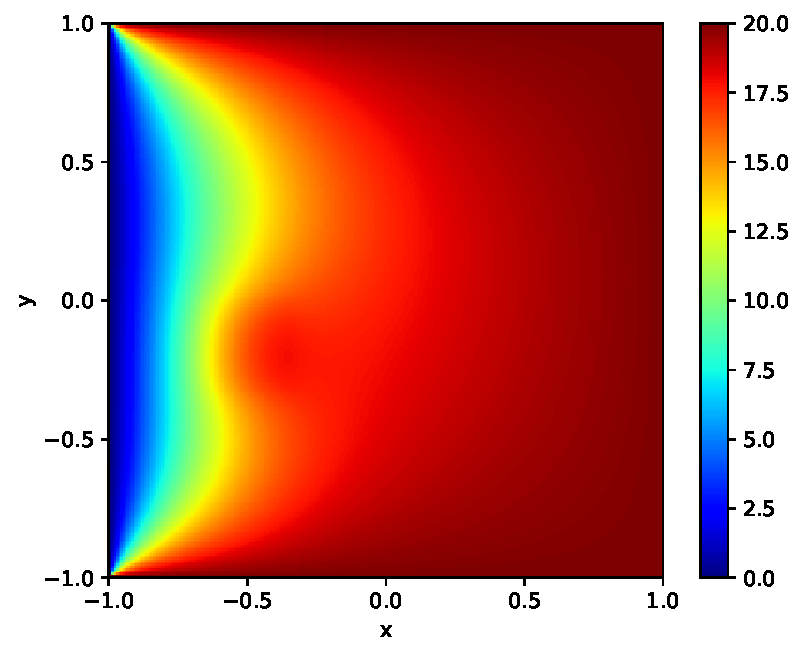
\includegraphics[width=.9\linewidth]{data_2/plots/gaus_con.pdf}
  \caption{Gauss-Seidel}
  \label{fig:}
\end{subfigure}%
\begin{subfigure}{.5\textwidth}
  \centering
  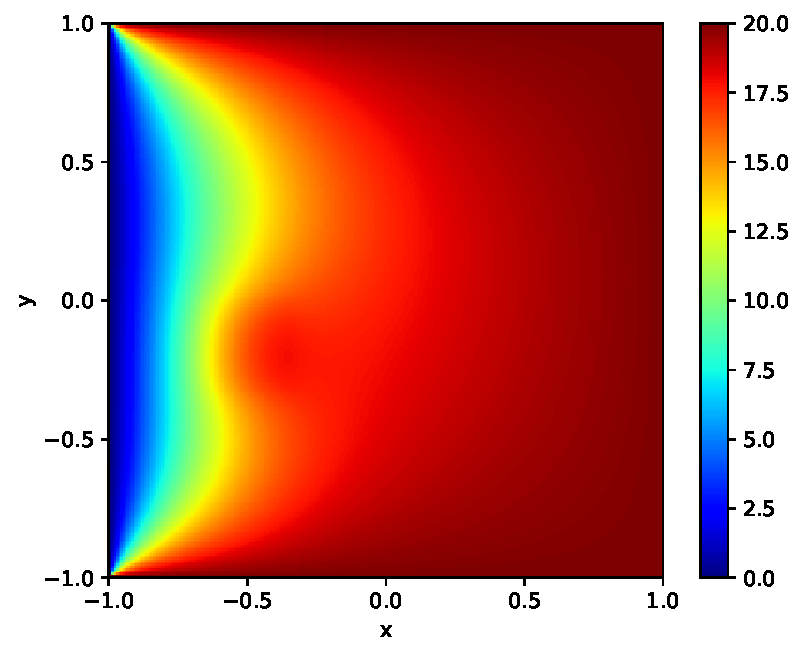
\includegraphics[width=.9\linewidth]{data_2/plots/jac_con.pdf}
  \caption{Jacobi}
  \label{fig:}
\end{subfigure}
\caption{Estimate of the function $u(x,y)$. The problem size of the illustrated heats are $N=256$. See table \ref{tab:seq_par} for further evaluation details.}
\label{fig:test}
\end{figure}

In table \ref{tab:seq_par}, details of the iterations of the two functions for problem sizes $N = 128$ and $256$ are shown. As expected, the memory usage in the Gauss-Seidel method is 2/3 of the Jacobi. This is due to the fact that three matrices are used in the Jacobi method, namely \texttt{f, u} and \texttt{u\_old}, whereas only \texttt{f} and \texttt{u} are needed in Gauss-Seidel. The number of iterations shows how many iterations are needed in order for $u(x,y)$ to converge. For both problem sizes, the Jacobi method needs almost twice as many iterations to reach convergence. In spite of this, the execution time is much larger in the case of Gauss-Seidel because the iterations are coupled, why the compiler optimizer fails to reduce runtime. This also means that fewer iterations and \texttt{mflops} are performed pr. second, as seen in the table. All together this information shows that if parallelization and smart memory allocation is implemented, there is a possibility of a larger performance gain for Gauss-Seidel than for Jacobi. On the other hand, Jacobi is easier parallelized as a result of the uncoupled iterations. 

\begin{table}[!th]
\centering
\begin{tabular}{ll|rrrrr}
&& Memory & Iterations & Duration & Iterations/s & mflops/s \\ \hline
\multirow{2}{*}{128}&\texttt{gauss\_con()}&262144&51225&4.79&10704&1754\\
&\texttt{jac\_seq\_con()}&393216&101831&1.76&57717&9456\\\hline
\multirow{2}{*}{256}&\texttt{gauss\_con()}&1048580&194176&73.38&2646&1734\\
&\texttt{jac\_seq\_con()}&1572860&390976&25.80&15153&9931\\
\end{tabular}
\caption{Comparison of the Jacobi method and Gauss-Seidel method.}
\label{tab:seq_par}
\end{table}

\subsection{OpenMP Jacobi}

The Jacobi method can be parallelized and run on multiple cores with shared memory using OpenMP. In the optimal setting the speed-up of increasing the number of cores is 1, i.e. using 2 cores instead of 1 should make the program run twice as fast. As discussed in the theory section OpenMP has several constructs which can be used to optimize the parallelization and ensure correctness. In the following sections, parallelized versions of the Jacobi method are implemented and continuously improved. For this purpose the number of iterations are fixed such that $k$ runs from 1 to \texttt{max\_iter} (with \texttt{max\_iter} = 5000) in order to best compare the efficiency of the different parallelized versions. Each version is run on 1, 4, 8, 16, and 24 threads for 4 different problem sizes $N \in \{256, 512, 1024, 2048\}$.

The first simple version will be used as a baseline.

\subsubsection{Version 1}

The first simple version has 2 parallel constructsm see algorithm \ref{alg:jac}: The first one contains a single-construct to make one of the threads extract the number of threads running the program. The second is nested within the while loop and contains a loop-construct such that the iterations from the outer for-loop (i.e. the rows) are distributed among the threads.

Figure \ref{fig:jac_comp_measure_v1} shows how increasing the number of threads for different problem sizes increases the number of flops per second. The gain is especially evident for $N = 512$ and $N = 1024$, while for $N = 2048$ there is no efficiency improvement when increasing the number of threads beyond $8$. This is explained by the fact that when $N$ is this size the problem does not fit within the 3 caches, hence
memory has to be fetched from the RAM which is significantly slower and hereby slows down the process.

In figure \ref{fig:scaling_mp_jac_v1} the speed-up for each problem size is compared to the theoretical speed-up. For problem sizes $256$, $512$, and $1024$ there is a clear correlation between problem size and speed-up, i.e. as the problem size increases so does the speed-up. This, however, is not the case for $N=2048$ which is as before most likely linked to the amount of needed memory. Since there are two sockets each running $12$ threads, they are forced to communicate when the number of threads exceeds 12 which could potentially slow down the process when the problem is large enough. 


\begin{figure}[H]
\centering
\begin{tikzpicture}[scale = 0.85]
\begin{axis}[
width=17cm, height=8cm,     % size of the image
grid = major,
grid style={dashed, gray!30},
xmode=log,log basis x=10,
ymin=0,    % start the diagram at this 
ymax=155000, % end   the diagram at this 
axis background/.style={fill=white},
ylabel=Mflops/s,
xlabel=Memory/kbytes,
legend pos=north east]
\addplot[mark=*, green] table [x=mem, y=mflops, col sep=comma]{data_2/plots/program_jac_mp_ncore_1.txt};
\addlegendentry{1 thread}
\addplot[mark=*, orange] table [x=mem, y=mflops, col sep=comma]{data_2/plots/program_jac_mp_ncore_4.txt};
\addlegendentry{4 threads}
\addplot[mark=*, blue] table [x=mem, y=mflops, col sep=comma]{data_2/plots/program_jac_mp_ncore_8.txt};
\addlegendentry{8 threads}
\addplot[mark=*, red] table [x=mem, y=mflops, col sep=comma]{data_2/plots/program_jac_mp_ncore_16.txt};
\addlegendentry{16 threads}
\addplot[mark=*, black] table [x=mem, y=mflops, col sep=comma]{data_2/plots/program_jac_mp_ncore_24.txt};
\addlegendentry{24 threads}
\end{axis}
\end{tikzpicture}
\caption{Jacobi version 1.}
\label{fig:jac_comp_measure_v1}
\end{figure}

\begin{figure}[H]
\centering
\begin{tikzpicture}[scale = 0.85]
\begin{axis}[
width=9cm, height=9cm,
grid = major,
grid style={dashed, gray!30},
xmin=0,
ymin=0,
ymax=24,
xmax=24,% end   the diagram at this 
/pgfplots/xtick={0,2,...,24},
/pgfplots/ytick={0,2,...,24},
axis background/.style={fill=white},
ylabel=S(P),
xlabel=P,
legend pos=north west]
\addplot[green, domain=0:25, no markers,samples=100] {x};
\addlegendentry{Theo.}
\addplot[mark=*, orange] table [x=ncore, y=SP, col sep=comma]{data_2/plots/program_jac_mp_SP_256.txt};
\addlegendentry{256}
\addplot[mark=*, blue] table [x=ncore, y=SP, col sep=comma]{data_2/plots/program_jac_mp_SP_512.txt};
\addlegendentry{512}
\addplot[mark=*, red] table [x=ncore, y=SP, col sep=comma]{data_2/plots/program_jac_mp_SP_1024.txt};
\addlegendentry{1024}
\addplot[mark=*, black] table [x=ncore, y=SP, col sep=comma]{data_2/plots/program_jac_mp_SP_2048.txt};
\addlegendentry{2048}
\end{axis} 
\end{tikzpicture}
\caption{Scaling Jacobi version 1.}
\label{fig:scaling_mp_jac_v1}
\end{figure}




\subsubsection{Version 2}

For version 2 the second parallel construct is moved out to include the while-loop as well, seen in algorithm \ref{alg:app_jac_mp_v23}. In the previous version the master thread distributed the iterations among the threads each time the while-loop counter $k$ was incremented by 1. Hence, there was a fork and a join of the threads for each $k$ from 1 to \texttt{max\_iter} which resulted in a lot of waiting time in between the actual computations. In this version the iterations are only distributed among the threads once which should decrease the waiting time. Now the pointers have to be swapped in parallel but this should only be done by one of the threads to avoid data racing. Therefore it is also crucial that the threads use the same iteration $k$ by declaring the variable as a \texttt{firstprivate}.

Figure \ref{fig:jac_comp_measure_v2} shows how the performance is now increased for each combination of problem size and number of threads (apart from 1 thread). The improvement is the most evident when using 24 threads, while it seems there is no improvement when using 1 thread. This makes sense since there is nothing running in parallel when using only 1 thread.

In figure \ref{fig:scaling_mp_jac_v2} it is hard to detect any improvement for problem sizes 256, 512, and 1024, while the speed-up for $N = 2048$ is a little better beyond 12 threads.

\begin{figure}[H]
\centering
\begin{tikzpicture}[scale = 0.85]
\begin{axis}[
width=17cm, height=8cm,     % size of the image
grid = major,
grid style={dashed, gray!30},
xmode=log,log basis x=10,
ymin=0,    % start the diagram at this 
ymax=155000, % end   the diagram at this 
axis background/.style={fill=white},
ylabel=Mflops/s,
xlabel=Memory/kbytes,
legend pos=north east]
\addplot[mark=*, green] table [x=mem, y=mflops, col sep=comma]{data_2/plots/program_jac_mp_v2_ncore_1.txt};
\addlegendentry{1 thread}
\addplot[mark=*, orange] table [x=mem, y=mflops, col sep=comma]{data_2/plots/program_jac_mp_v2_ncore_4.txt};
\addlegendentry{4 threads}
\addplot[mark=*, blue] table [x=mem, y=mflops, col sep=comma]{data_2/plots/program_jac_mp_v2_ncore_8.txt};
\addlegendentry{8 threads}
\addplot[mark=*, red] table [x=mem, y=mflops, col sep=comma]{data_2/plots/program_jac_mp_v2_ncore_16.txt};
\addlegendentry{16 threads}
\addplot[mark=*, black] table [x=mem, y=mflops, col sep=comma]{data_2/plots/program_jac_mp_v2_ncore_24.txt};
\addlegendentry{24 threads}
\end{axis} 
\end{tikzpicture}
\caption{Jacobi version 2.}
\label{fig:jac_comp_measure_v2}
\end{figure}


\begin{figure}[H]
\centering
\begin{tikzpicture}[scale = 0.85]
\begin{axis}[
width=9cm, height=9cm,
grid = major,
grid style={dashed, gray!30},
xmin=0,
ymin=0,
ymax=24,
xmax=24,% end   the diagram at this 
/pgfplots/xtick={0,2,...,24},
/pgfplots/ytick={0,2,...,24},
axis background/.style={fill=white},
ylabel=S(P),
xlabel=P,
legend pos=north west]
\addplot[green, domain=0:25, no markers,samples=100] {x};
\addlegendentry{Theo.}
\addplot[mark=*, orange] table [x=ncore, y=SP, col sep=comma]{data_2/plots/program_jac_mp_v2_SP_256.txt};
\addlegendentry{256}
\addplot[mark=*, blue] table [x=ncore, y=SP, col sep=comma]{data_2/plots/program_jac_mp_v2_SP_512.txt};
\addlegendentry{512}
\addplot[mark=*, red] table [x=ncore, y=SP, col sep=comma]{data_2/plots/program_jac_mp_v2_SP_1024.txt};
\addlegendentry{1025}
\addplot[mark=*, black] table [x=ncore, y=SP, col sep=comma]{data_2/plots/program_jac_mp_v2_SP_2048.txt};
\addlegendentry{2048}
\end{axis} 
\end{tikzpicture}
\caption{Scaling Jacobi version 2.}
\label{fig:scaling_mp_jac_v2}
\end{figure}




\subsubsection{Version 3}

For the final version the Jacobi method itself is the same as version 2, but this time the initialization of the matrices is also parallelized. Hence, the data is pre-distributed among the threads to make it more accessible when running the actual program. 

In figure \ref{fig:jac_comp_measure_v3} it is once again obvious that the larger of the problem sizes are the ones to exploit the further parallelization the most. Especially $N = 2048$ utilizes the parallelized initialization of the matrices, which makes sense given the large memory consumption.

By considering figure \ref{fig:scaling_mp_jac_v3} it is clear that the problem sizes $256$ and $512$ experience the best improvement of speed-up, while $N=1024$ seems to be unchanged.

\begin{figure}[H]
\centering
\begin{tikzpicture}[scale = 0.85]
\begin{axis}[
width=17cm, height=8cm,     % size of the image
grid = major,
grid style={dashed, gray!30},
xmode=log,log basis x=10,
ymin=0,    % start the diagram at this 
ymax=155000, % end   the diagram at this 
axis background/.style={fill=white},
ylabel=Mflops/s,
xlabel=Memory/kbytes,
legend pos=north east]
\addplot[mark=*, green] table [x=mem, y=mflops, col sep=comma]{data_2/plots/program_jac_mp_v3_ncore_1.txt};
\addlegendentry{1 thread}
\addplot[mark=*, orange] table [x=mem, y=mflops, col sep=comma]{data_2/plots/program_jac_mp_v3_ncore_4.txt};
\addlegendentry{4 threads}
\addplot[mark=*, blue] table [x=mem, y=mflops, col sep=comma]{data_2/plots/program_jac_mp_v3_ncore_8.txt};
\addlegendentry{8 threads}
\addplot[mark=*, red] table [x=mem, y=mflops, col sep=comma]{data_2/plots/program_jac_mp_v3_ncore_16.txt};
\addlegendentry{16 threads}
\addplot[mark=*, black] table [x=mem, y=mflops, col sep=comma]{data_2/plots/program_jac_mp_v3_ncore_24.txt};
\addlegendentry{24 threads}
\end{axis} 
\end{tikzpicture}
\caption{Jacobi version 3.}
\label{fig:jac_comp_measure_v3}
\end{figure}



\begin{figure}[H]
\centering
\begin{tikzpicture}[scale = 0.85]
\begin{axis}[
width=9cm, height=9cm,
grid = major,
grid style={dashed, gray!30},
xmin=0,
ymin=0,
ymax=24,
xmax=24,% end   the diagram at this 
/pgfplots/xtick={0,2,...,24},
/pgfplots/ytick={0,2,...,24},
axis background/.style={fill=white},
ylabel=S(P),
xlabel=P,
legend pos=north west]
\addplot[green, domain=0:25, no markers,samples=100] {x};
\addlegendentry{Theo.}
\addplot[mark=*, orange] table [x=ncore, y=SP, col sep=comma]{data_2/plots/program_jac_mp_v3_SP_256.txt};
\addlegendentry{256}
\addplot[mark=*, blue] table [x=ncore, y=SP, col sep=comma]{data_2/plots/program_jac_mp_v3_SP_512.txt};
\addlegendentry{512}
\addplot[mark=*, red] table [x=ncore, y=SP, col sep=comma]{data_2/plots/program_jac_mp_v3_SP_1024.txt};
\addlegendentry{1024}
\addplot[mark=*, black] table [x=ncore, y=SP, col sep=comma]{data_2/plots/program_jac_mp_v3_SP_2048.txt};
\addlegendentry{2048}
\end{axis} 
\end{tikzpicture}
\caption{Scaling Jacobi version 3.}
\label{fig:scaling_mp_jac_v3}
\end{figure}

%DET ER YDERST fedt at se 2048 hvor P er 1,2 og 4





\subsubsection{Comparison}

In figure \ref{fig:jac_comp_measure_v123} the efficiency of the 3 different OpenMP Jacobi methods are compared for 4 different problem sizes (the same as before) using 8 and 16 cores. Version 1 is outperformed by version 2 and 3 using both 8 and 16 threads. With 8 threads version 2 and 3 are practically indistinguishable, while using 16 threads the best performing version alternates between 2 and 3 depending on the problem size.

\begin{figure}[H]
\centering
\begin{tikzpicture}[scale = 1]
\begin{axis}[
width=17cm, height=8cm,     % size of the image
grid = major,
grid style={dashed, gray!30},
xmode=log,log basis x=10,
ymin=0,    % start the diagram at this 
ymax=155000, % end   the diagram at this 
axis background/.style={fill=white},
ylabel=Mflops/s,
xlabel=Memory/kbytes,
legend pos=north east]
\addplot[mark=*, purple] table [x=mem, y=mflops, col sep=comma]{data_2/plots/program_jac_mp_ncore_8.txt};
\addlegendentry{v1\_8}
\addplot[mark=*, orange] table [x=mem, y=mflops, col sep=comma]{data_2/plots/program_jac_mp_v2_ncore_8.txt};
\addlegendentry{v2\_8}
\addplot[mark=*, green] table [x=mem, y=mflops, col sep=comma]{data_2/plots/program_jac_mp_v3_ncore_8.txt};
\addlegendentry{v3\_8}


\addplot[mark=*, red] table [x=mem, y=mflops, col sep=comma]{data_2/plots/program_jac_mp_ncore_16.txt};
\addlegendentry{v1\_16}
\addplot[mark=*, black] table [x=mem, y=mflops, col sep=comma]{data_2/plots/program_jac_mp_v2_ncore_16.txt};
\addlegendentry{v2\_16}
\addplot[mark=*, blue] table [x=mem, y=mflops, col sep=comma]{data_2/plots/program_jac_mp_v3_ncore_16.txt};
\addlegendentry{v3\_16}

\end{axis}
\end{tikzpicture}
\caption{Jacobi version 1, 2 and 3 for 8 and 16 threads.}
\label{fig:jac_comp_measure_v123}
\end{figure}

\subsection{Mandelbrot}

The scaling behaviour of the Jacobi method and of the Mandelbrot algorithm is given in figure \ref{fig:scaling_comp_opt} and in figure \ref{fig:scaling_non_comp_opt} with and without compiler optimization flags repectively.

The four methods have been evaluated for $N=1024$ and with $ max_{iter} = 5000$.

\begin{figure}[H]
\begin{subfigure}{.5\textwidth}
\centering
\begin{tikzpicture}[scale = 1]
\begin{axis}[
width=8cm, height=8cm,
grid = major,
grid style={dashed, gray!30},
xmin=0,
ymin=0,
ymax=24,
xmax=24,% end   the diagram at this 
/pgfplots/xtick={0,2,...,24},
/pgfplots/ytick={0,2,...,24},
axis background/.style={fill=white},
ylabel=S(P),
xlabel=P,
legend pos=north west]
\addplot[green, domain=0:25, no markers,samples=100] {x};
\addlegendentry{Theo.}
\addplot[mark=*, black] table [x=ncore, y=SP, col sep=comma]{data_2/plots/program_mandel.txt};
\addlegendentry{Mandel}
\addplot[mark=*, red] table [x=ncore, y=SP, col sep=comma]{data_2/plots/program_jac_mp_SP.txt};
\addlegendentry{Jacobi\_v1}
\addplot[mark=*, blue] table [x=ncore, y=SP, col sep=comma]{data_2/plots/program_jac_mp_v2_SP.txt};
\addlegendentry{Jacobi\_v2}
\addplot[mark=*, orange] table [x=ncore, y=SP, col sep=comma]{data_2/plots/program_jac_mp_v3_SP.txt};
\addlegendentry{Jacobi\_v3}
\end{axis} 
\end{tikzpicture}
\caption{Optimized}
\label{fig:scaling_comp_opt}
\end{subfigure}%
\begin{subfigure}{.5\textwidth}
\centering
\begin{tikzpicture}[scale = 1]
\begin{axis}[
width=8cm, height=8cm,
grid = major,
grid style={dashed, gray!30},
xmin=0,
ymin=0,
ymax=24,
xmax=24,% end   the diagram at this 
/pgfplots/xtick={0,2,...,24},
/pgfplots/ytick={0,2,...,24},
axis background/.style={fill=white},
ylabel=S(P),
xlabel=P,
legend pos=north west]
\addplot[green, domain=0:25, no markers,samples=100] {x};
\addlegendentry{Theo.}
\addplot[mark=*, black] table [x=ncore, y=SP, col sep=comma]{data_2/plots/program_mandel_non.txt};
\addlegendentry{Mandel\_non}
\addplot[mark=*, red] table [x=ncore, y=SP, col sep=comma]{data_2/plots/program_jac_mp_SP_non.txt};
\addlegendentry{Jacobi\_v1\_non}
\addplot[mark=*, blue] table [x=ncore, y=SP, col sep=comma]{data_2/plots/program_jac_mp_v2_SP_non.txt};
\addlegendentry{Jacobi\_v2\_non}
\addplot[mark=*, orange] table [x=ncore, y=SP, col sep=comma]{data_2/plots/program_jac_mp_v3_SP_non.txt};
\addlegendentry{Jacobi\_v3\_non}
\end{axis} 
\end{tikzpicture}
\caption{Non optimized}
\label{fig:scaling_non_comp_opt}
\end{subfigure}
\caption{The plots shows the scaling as function of number of threads P with following compiler flags: \texttt{-fast -xopenmp} and \texttt{-xopenmp=noopt} for \ref{fig:scaling_comp_opt} and \ref{fig:scaling_non_comp_opt} respectively.}
%\label{fig:test}
\end{figure}

There is a slight difference between the three versions of the Jacobi method when not using the mentioned compiler optimization flags, see figure \ref{fig:scaling_non_comp_opt}. The three versions follows each other for a given $P$ except for $P=24$.

It can be concluded that the current implementation of the Mandelbrot algorithm (algo. \ref{alg:app_mandel}) does not scale as the implementations of the Jacobi method, see table \ref{tab:avergae_f} where $f$ have been derived from eq. \ref{eq:SPp}.
An explanation for the scaling of the Mandelbrot is the unbalanced work load in the while loop for the assigned threads. A solution to this could be dynamic scheduling of the work balance.

Table \ref{tab:avergae_f} reports the average values of $f$ for the curves in figure \ref{fig:scaling_comp_opt} and figure \ref{fig:scaling_non_comp_opt}. $f$ have been derived from eq. \ref{eq:SPp}.

\begin{table}[H]
\centering
\begin{tabular}{l|cc}
Algo. & $f_{opt}$ & $f_{non}$  \\\hline
\texttt{manddel()} & 0.730 & 0.726\\
\texttt{jac\_mp()} & 0.976 & 0.972\\
\texttt{jac\_mp\_v2()} & 0.974 & 0.974\\
\texttt{jac\_mp\_v3()} & 0.976 & 0.980\\
\end{tabular}
\caption{Average value of $f$ for each algorithm. The values in the second column corresponds to figure \ref{fig:scaling_comp_opt} and the third column corresponds to figure \ref{fig:scaling_non_comp_opt}. }
\label{tab:avergae_f}
\end{table}
The max speed-up limit for \texttt{jac\_mp\_v3()} is $S_{max}(0.976)=\left\lfloor  41 \right\rfloor$. The max speed-up limit for \texttt{mandel()} is $S_{max}(0.730)=\left\lfloor  3\right\rfloor$, see eq. \ref{eq:SPmax}.


\section{Conclusion}
The sequential codes for the Jacobi and Gauss-Seidel methods showed that while the Gauss-Seidel method needs less iterations for the solution to converge, it is still much slower than Jacobi. This is because more floating point operations are performed pr. second in Jacobi. From the analysis of the performance of the sequential programs it was found that parallelization and smarter data allocation could enhance the performance of both methods, but that the possible gain might be higher for using Gauss-Seidel, due to convergence being reached after fewer iterations and the fact that this method uses less memory. 


As previously discussed the parallelized third version of the Jacobi method clearly improved the efficiency (number of flops per second) compared to the first and second version. The improvement of the speed-up is not that evident for the problem sizes 256, 512, and 1024, but when the problem doesn't fit within the first three caches and has to be stored in the RAM, there is some gain in speed-up when optimizing the parallelization – both with respect to the Jacobi method itself and the initialization of the matrices.

For future work it could be beneficial to implement the \texttt{NUMA} control policy.

\begin{center}
{{\Large \sc High-Performance Computing}}
\end{center}
\rule{\textwidth}{1pt}
\begin{description}
\item[Student name and id:] % Marie Mørk \{s112770\} %Anders Launer Bæk \{s160159\} %\textcolor{red}{Marie Mørk \{s112770\} Anja Liljedahl Christensen\{s162876\}
 Andreas Vedel Jantzen \{s162858\}
 %Anders Launer Bæk \{s160159\}}
\item[Collaborators:] Anja Liljedahl Christensen\{s162876\} {Marie Mørk \{s112770\}} Anders Launer Bæk \{s160159\} %Andreas Vedel Jantzen \{s162858\} Anders Launer Bæk \{s160159\} {Marie Mørk \{s112770\} Anja Liljedahl Christensen\{s162876\}
 %Andreas Vedel Jantzen \{s162858\}
 %Anders Launer Bæk \{s160159\}}
\item[Hand-in:] GPU Computing
\end{description}
\rule{\textwidth}{1pt}

\section{Summary}
In the report, the problems from assignment 1 and 2 are solved by implementing algorithms that make use of GPUs. Six different algorithms for performing matrix multiplication are implemented. This includes a GPU library function. The performance of the algorithms are compared and a speed-up calculated using the cBLAS DGEMM subroutine as reference. The best performing algorithm is found to be \texttt{gpu5}, which one thread on the device to calculate each element in the resulting matrix $C$, and exploits shared memory. In the chosen range of problem sizes, this algorithm performs even better than the GPU library function, cublasDgemm. \\
Three Jacobi methods for solving the Poisson problem, with different levels of utilization of the GPU have also been implemented. The performance of these has been compared to the fastest CPU implementation from assignment 2. The best performing GPU implementation has a speed-up of $\approx \times 16$.

\section{Statement of the problem}
In this assignment GPU computing is used to solve the problems from the two earlier reports in order to see if GPU computing enhance the performance. The report is therefore split in two parts; one concerning matrix-matrix multiplication, and the other on the Poisson problem. \\ \ \\
\textbf{Matrix-matrix multiplication}\\
In the part about matrix-matrix multiplication, the dimensions of the matrices are the same as in Assignment 1, see figure \ref{fig:mat_or}. The performance of the implemented algorithms are to be compared with the cBLAS DGEMM subroutine used in Assignment 1. \\
\begin{figure}[H]
    \centering
    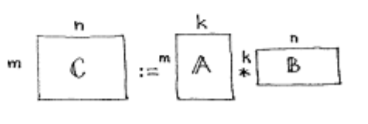
\includegraphics{contents/pics_1/matmult.PNG}
    \caption{Visualization of the matrix orientation. The picture is borrowed from the description of Assignment 1.}
    \label{fig:mat_or}
\end{figure}
\noindent Six different algorithms for matrix-matrix multiplications using GPUs are to be implemented. In the following, a short description of the algorithms is provided listed by their function calls. 
\begin{itemize}
    \item \texttt{lib}: Multithreaded cBLAS DGEMM subroutine as reference.
    \item \texttt{gpu1}: Using a single thread. 
    \item \texttt{gpu2}: Using one thread pr. element in matrix C.
    \item \texttt{gpu3}: Using one thread pr. 2 elements in matrix C. The optimal placement of the elements relative to each other is to be found.
    \item \texttt{gpu4}: Computing more than two elements in the C matrix pr. thread. The optimal placement of the elements relative to each other and number of elements is to be found.
    \item \texttt{gpu5}: Based upon the implementation linked to in the assignment description and modified to be compatible with the driver.
    \item \texttt{gpulib}: Implementation of the cuBLAS DGEMM subroutine.
\end{itemize} \ \\
\textbf{Poisson Problem}\\
The Poisson problem from assignment 2 will be solved using the Jacobi method. Three different algorithms will be implemented:
\begin{itemize}
    \item \texttt{jac\_cpu}: Best OpenMP function of the Jacobia function as reference.
    \item \texttt{jac\_gpu1}: A sequential version using one thread and doing one iteration pr kernel launch.
    \item \texttt{jac\_gpu2}: A naive version using one thread pr. grid point and only rely on global memory.
    \item \texttt{jac\_gpu3}: Multiple GPU version, in which the interior points are to be updated from global memory and the boarder points between the two regions is read as peer values from the other GPU.  
\end{itemize}
The kernels used are analyzed by the NVIDIA Visual Profiler (\texttt{nvvp}) in both parts of the assignment. 

\section{Hardware and software}
Specifications of the test environment are listed below:
\begin{itemize}
\item CPU information
\begin{itemize}
\item CPU(s):                24
\item Thread(s) per core:    1
\item Core(s) per socket:    12
\item Vendor ID:             GenuineIntel
\item CPU family:            6
\item Model:                 85
\item Model name:            Intel(R) Xeon(R) Gold 6126 CPU @ \item 2.60GHz
\item CPU MHz:               2600.000
\item L1 (d / i) cache:             32K
\item L2 cache:              1024K
\item L3 cache:              19712K
\end{itemize}

\item GPU information
\begin{itemize}
\item NVIDIA TESLA V100 FOR PCle x2
\item NVIDIA-SMI 387.26
\item Driver Version: 387.26
\end{itemize}
\item Compilers
\begin{itemize}
\item The SunCC compiler have been applied with followings flags: \texttt{-fast -xopenmp -xrestrict} for OpenMP reference in the Poisson problem.
\item \texttt{nnv} is used for default compilation of the cuda code.
\end{itemize}
\end{itemize}




\section{Theory}
%In this assignment a GPU will be used to solve problems, but why are GPUs important in HPC? For this to make sense lets go to the differences of how a GPU and a CPU process tasks. Very basic, a 
One of the advantages of using a GPU instead of a CPU is that while a CPU has few cores, a GPU has thousands of smaller more efficient cores, that can work simultaneously. This results in a much higher amount of floating point operations and a much higher bandwidth, though the GPU cores can only perform simple operations, and the CPU cores can be assigned to different and more complicated operations \cite{C4}.\\

\noindent The computations will be performed on a NVIDIA TESLA V100 GPU, hence the NVIDIA GPU optimized language CUDA will be used.\\

\noindent For medium to large matrices, matrix-matrix multiplication has the potential to be a compute-bound operation. The Jacobi method, on the other hand, is a memory-bound operation. %This report will examine the bounding, using the NVIDIA analysis tool \texttt{nvvp}. 

%Something on how the memory model works on GPUs and how this can be optimised. 

%Speed up

%Performance 

%SOmething about the nvvp profiler and how we use this

\newpage

\section{Matrix-matrix multiplication}
In this section the algorithms, results, and analysis of the kernels used for matrix-matrix multiplication will be presented. The performance of the algorithms will be compared with each other and the CBLAS library DGEMM subroutine, which was implemented in the function \texttt{matmult\_lib} in Assignment 1. The implementation of this algorithm will not be described again in this report, but the code is listed in the appendix, see algorithm \ref{alg:CPU_lib}.\\
Please note that the speed-ups are calculated based on the old driver on DTU Inside, which only uses 4 threads. Due to this, the calculated speed-ups are overestimated. Unfortunately, there was not sufficient time to update all the results.

\subsection{\texttt{gpu1}}
As already mentioned, in the implementation of \texttt{matmult\_gpu1} the kernel is launched with a single thread. The implementation of the algorithm (both the CPU function and the kernel) is listed in algorithm \ref{alg:gpu1}.\\

\lstinputlisting[label={alg:gpu1},caption={\texttt{matmult\_gpu1}, CPU function and kernel.},style=CStyle, 
linerange={21-73}]{code_3/func_cu.tex}

\noindent The performance of \texttt{matmult\_gpu1} will be compared to the CPU CBLAS subroutine DGEMM. Performance is only measured for small matrix sizes, in this case four square matrices of sizes N = M = K = 32, 64, 96, and 128. Figure \ref{fig:compare_gpu1} shows the number of floating point operations pr. second in Mflops/s for the four matrix sizes.\\

\noindent The figure shows that \texttt{matmult\_gpu1} is significantly slower than the optimized CPU library function DGEMM. This is as expected, as the GPU version only uses one thread, which means that the version is sequential and thereby does not take advantage of parallelism of the threads in the GPU. In addition to this, \texttt{gpu1} uses time for copying memory between the host and the device. The CPU function implementation on the other hand, is optimized using parallel programming ect. which makes it much faster. \\

\noindent In figure \ref{fig:speed_gpu1}, the speed-up of \texttt{gpu1} compared to \texttt{lib} is shown. As it is already apparent from figure \ref{fig:compare_gpu1}, the speed-up is below 1, meaning that the CPU version is faster than the GPU. \\

\noindent Performance of the GPUs is also evaluated using the \texttt{nvprof} command in the shell. For \texttt{gpu1}, the GPU summary shows that $99.98\%-100\%$ of the time used for executing the GPU function is used in the kernel, whereas very little time is used for copying between host and device. This shows that in order for the algorithm to have a better performance, the computations within the kernels should be optimized. \\


\begin{figure}[H]
\centering
\begin{tikzpicture}[scale = 0.85]
\begin{axis}[
width=17cm, height=8cm,     % size of the image
grid = major,
grid style={dashed, gray!30},
xmode=log,log basis x=10,
%ymin=0,    % start the diagram at this 
%ymax=155000, % end   the diagram at this 
axis background/.style={fill=white},
ylabel=Mflops/s,
xlabel=Memory/kbytes,
legend pos=north west]
\addplot[mark=*, orange] table [x=mem, y=mflops, col sep=comma]{data_3/mat/lib_small.txt};
\addlegendentry{\texttt{lib()}}
\addplot[mark=*, blue] table [x=mem, y=mflops, col sep=comma]{data_3/mat/gpu1.txt};
\addlegendentry{\texttt{gpu1()}}
\end{axis} 
\end{tikzpicture}
\caption{Comparison of \texttt{gpu1} and \texttt{lib}.}
\label{fig:compare_gpu1}
\end{figure}

\begin{figure}[H]
\centering
\begin{tikzpicture}[scale = 0.85]
\begin{axis}[
width=17cm, height=8cm,     % size of the image
grid = major,
grid style={dashed, gray!30},
xmode=log,log basis x=10,
%ymin=0,    % start the diagram at this 
%ymax=155000, % end   the diagram at this 
axis background/.style={fill=white},
ylabel=Speed-up,
xlabel=Memory/kbytes,
legend pos=north west]
\addplot[mark=*, orange] table [x=mem, y=speed, col sep=comma]{data_3/mat/speed_gpu1.txt};
\addlegendentry{Speed-up}
\end{axis} 
\end{tikzpicture}
\caption{Speed up of \texttt{gpu1} compared to \texttt{lib}.}
\label{fig:speed_gpu1}
\end{figure}


\subsection{\texttt{gpu2}}
The kernel for \texttt{matmult\_gpu2} is listed in algorithm \ref{alg:gpu2K}, while the changes in the launch from the CPU function is listed in \ref{alg:gpu2L}. This time each thread computes one element of $C$: the thread with global thread id $(i,j)$ computes element $(i,j)$ in $C$. If there are more threads than elements in $C$ the remaining threads will not compute anything.\\

\lstinputlisting[label={alg:gpu2K},caption={\texttt{matmult\_gpu2} kernel.},style=CStyle, linerange={76-89}]{code_3/func_cu.tex}
\lstinputlisting[label={alg:gpu2L},caption={\texttt{matmult\_gpu2} launch of kernel.},style=CStyle, linerange={111-114}]{code_3/func_cu.tex}

\noindent Matrix sizes used for the comparison between \texttt{gpu2} and the CPU library function is set to be multiples of 16, such that the same matrix sizes can be used to compare with \texttt{gpu5} in a later section. We choose square matrices with dimensions 800, 1600, 2400, 3200, 4000, 4800, and 5600. In figure \ref{fig:compare_gpu2}, Mflops/s as a function of problem size is shown for \texttt{gpu2} and \texttt{lib}. Comparing the two graphs, the advantages of using GPUs is now clearly visible and \texttt{gpu2} is faster than \texttt{lib} for all matrix sizes considered. \\
\begin{figure}[H]
\centering
\begin{tikzpicture}[scale = 0.85]
\begin{axis}[
width=17cm, height=8cm,     % size of the image
grid = major,
grid style={dashed, gray!30},
xmode=log,log basis x=10,
%ymin=0,    % start the diagram at this 
%ymax=155000, % end   the diagram at this 
axis background/.style={fill=white},
ylabel=Mflops/s,
xlabel=Memory/kbytes,
legend pos=north west]
\addplot[mark=*, orange] table [x=mem, y=mflops, col sep=comma]{data_3/mat/lib.txt};
\addlegendentry{\texttt{lib()}}
\addplot[mark=*, blue] table [x=mem, y=mflops, col sep=comma]{data_3/mat/gpu2.txt};
\addlegendentry{\texttt{gpu2()}}
\end{axis} 
\end{tikzpicture}
\caption{Comparison of \texttt{gpu2} and \texttt{lib}.}
\label{fig:compare_gpu2}
\end{figure}
\noindent The speed-up is computed from mflops/s and reported in figure \ref{fig:speed_gpu2} for the chosen matrix sizes. It is seen that the speed-up rises with problem size up until matrices with dimensions higher than 3200. For larger matrices, the speed-up stays constant at around 4x. 

\begin{figure}[H]
\centering
\begin{tikzpicture}[scale = 0.85]
\begin{axis}[
width=17cm, height=8cm,     % size of the image
grid = major,
grid style={dashed, gray!30},
xmode=log,log basis x=10,
%ymin=0,    % start the diagram at this 
%ymax=155000, % end   the diagram at this 
axis background/.style={fill=white},
ylabel=Speed-up,
xlabel=Memory/kbytes,
legend pos=north west]
\addplot[mark=*, orange] table [x=mem, y=speed, col sep=comma]{data_3/mat/speed_gpu2.txt};
\addlegendentry{Speed-up}
\end{axis} 
\end{tikzpicture}
\caption{Speed up of \texttt{gpu2} compared to \texttt{lib}.}
\label{fig:speed_gpu2}
\end{figure}

\noindent Using the call \texttt{nvprof --print-gpu-summary} in the shell, the different parts of the GPU function is timed. In table \ref{tab:time_gpu2}, the percentage used in the kernel, on copying from host to device, and from device to host is listed. For smaller problem sizes, the percentage of the total execution time used in the kernel is smaller than for large problems. It is to expect, as fewer calculations are needed for small matrices, while the memory still needs to be transferred between host and device.

\begin{table}[H]
    \centering
    \begin{tabular}{c|c c c}
         Problem size&Kernel & HtoD & DtoH \\ \hline
         800 & 81.63\% & 12.55\% & 5.82\% \\
         1600 & 89.86\% & 6.92\% & 3.23\% \\
         2400 & 92.93\% & 4.82\% & 2.25\% \\
         3200 & 94.11\% & 4.01\% & 1.88\% \\
         4000 &95.19\% & 3.28\% & 1.53\%\\
         4800 & 95.95\% & 2.76\% & 1.29\% \\
         5600 & 96.51\% & 2.38\%& 1.11\%
    \end{tabular}
    \caption{Time spend on Kernel, HtoD and DtoH in the kernel of \texttt{gpu2} for the chosen problem sizes.}
    \label{tab:time_gpu2}
\end{table}

\subsection{\texttt{gpu3}}
In \texttt{gpu3}, each thread is to compute 2 elements in $C$. To do this, a stride introduced in the algorithm. The function is tested for the stride in both the $x$ and the $y$ direction for large matrices. A stride in $y$ is found to be the fastest, hence the second element in $C$ which is computed by the thread is the neighbor below the first element. This makes sense since in this way the threads access memory coalesced. Furthermore this way a single thread will access one column in $B$ and two rows in $A$ in order to compute the two elements in $C$. As memory storage in $C$ is row-major, it is expected that accessing two rows and one column is faster than the opposite for each thread. The kernel for this implementation is listed in algorithm \ref{alg:gpu3K}, while the changes in the launch from the CPU function is listed in algorithm \ref{alg:gpu3L}.\\
\noindent Compared to the previous two kernels \texttt{gpu3\_kernel} takes an extra argument which is the stride in the $y$ ($i$) direction. Since each thread has to compute 2 elements, \texttt{stride} is set to 2 when the kernel is launched, see algorithm \ref{alg:gpu3L}. In algorithm \ref{alg:gpu3K} the thread with global thread id $(i,j)$ will then compute element $(i\cdot 2, j)$ and $(i\cdot 2 + 1, j)$ of $C$. \\

\lstinputlisting[label={alg:gpu3K},caption={\texttt{gpu3} kernel.},style=CStyle, linerange={132-147}]{code_3/func_cu.tex}
\lstinputlisting[label={alg:gpu3L},caption={\texttt{gpu3} launch of kernel.},style=CStyle, linerange={170-173}]{code_3/func_cu.tex}

\noindent Again, the performance of the algorithm is compared to that of \texttt{lib}. In figure \ref{fig:compare_gpu3}, Mflops/s is shown for different problem sizes. For the largest problem size, \texttt{gpu3} computes almost twice as many Mflops/s as \texttt{gpu2}. This means that the speed up compared to the CPU version is higher for \texttt{gpu3}.
\begin{figure}[H]
\centering
\begin{tikzpicture}[scale = 0.85]
\begin{axis}[
width=17cm, height=8cm,     % size of the image
grid = major,
grid style={dashed, gray!30},
xmode=log,log basis x=10,
%ymin=0,    % start the diagram at this 
%ymax=155000, % end   the diagram at this 
axis background/.style={fill=white},
ylabel=Mflops/s,
xlabel=Memory/kbytes,
legend pos=north west]
\addplot[mark=*, orange] table [x=mem, y=mflops, col sep=comma]{data_3/mat/lib.txt};
\addlegendentry{\texttt{lib()}}
\addplot[mark=*, blue] table [x=mem, y=mflops, col sep=comma]{data_3/mat/gpu3.txt};
\addlegendentry{\texttt{gpu3()}}
\end{axis} 
\end{tikzpicture}
\caption{Comparison of \texttt{gpu3} and \texttt{lib}.}
\label{fig:compare_gpu3}
\end{figure}

\noindent In figure \ref{fig:speed_gpu3}, the calculated speed-ups are shown for the chosen problem sizes. The graph shows the same tendency as the speed-up for \texttt{gpu2} namely that the speed up cease to increase for problem sizes larger than 3200. The speed-up is almost doubled compared to \texttt{gpu2}.

\begin{figure}[H]
\centering
\begin{tikzpicture}[scale = 0.85]
\begin{axis}[
width=17cm, height=8cm,     % size of the image
grid = major,
grid style={dashed, gray!30},
xmode=log,log basis x=10,
%ymin=0,    % start the diagram at this 
%ymax=155000, % end   the diagram at this 
axis background/.style={fill=white},
ylabel=Speed-up,
xlabel=Memory/kbytes,
legend pos=north west]
\addplot[mark=*, orange] table [x=mem, y=speed, col sep=comma]{data_3/mat/speed_gpu3.txt};
\addlegendentry{Speed-up}
\end{axis} 
\end{tikzpicture}
\caption{Speed up of \texttt{gpu3} compared to \texttt{lib}.}
\label{fig:speed_gpu3}
\end{figure}

\subsection{\texttt{gpu4}}
In the previous version each thread computed 2 elements of $C$, but now the number of elements for each thread has to be more than 2. It is immediately ruled out to assign elements in more than 1 column of $C$ for each thread (since it is faster for the threads to access memory coalesced), hence the question is: how many element in 1 column (directly on top of each other) should each thread compute. This is investigated by using the matrix sizes $M=N=K=5000$ and trying out different strides in the $y$ direction. The kernel is listed in algorithm \ref{alg:gpu4K}, while the changes in the launch from the CPU function is listed in algorithm \ref{alg:gpu4L}.\\

\lstinputlisting[label={alg:gpu4K},caption={\texttt{gpu4} kernel.},style=CStyle, linerange={191-212}]{code_3/func_cu.tex}
\lstinputlisting[label={alg:gpu4L},caption={\texttt{gpu4} launch of kernel.},style=CStyle, linerange={235-238}]{code_3/func_cu.tex}

\noindent In figure \ref{fig:gpu4_opt} below the GPU time is recorded for small values of \texttt{stride\_m}, i.e. from 3 to 64, and in figure \ref{fig:gpu4_opt2} the GPU time is recorded for larger values of \texttt{stride\_m}. The size of both strides (\texttt{stride\_n} in the $x$ direction and \texttt{stride\_m} in the $y$ direction) are given as arguments from the command line. This might explain the strange behavior of the GPU time. When the strides are not predefined at compile time, memory is not allocated optimally. Hence, the registers of the threads are not fully exploited. From the plots below, the GPU time is minimal when each thread computes 6 elements, though it is hard to see.  

\begin{figure}[H]
\centering
\begin{tikzpicture}[scale = 0.85]
\begin{axis}[
width=17cm, height=8cm,     % size of the image
grid = major,
grid style={dashed, gray!30},
%xmode=log,log basis x=10,
ymin=0.6,    % start the diagram at this 
ymax=1.35, % end   the diagram at this 
axis background/.style={fill=white},
ylabel=Time in s.,
xlabel=stride\_m,
legend pos=north west]
\addplot[mark=*, orange] table [x=stride_m, y=time, col sep=comma]{data_3/gpu4_opt2.txt};
%\addlegendentry{\texttt{lib()}}
% \addplot[mark=*, blue] table [x=mem, y=mflops, col sep=comma]{data_3/mat/gpu1.txt};
%\addlegendentry{\texttt{gpu4()}}
\end{axis} 
\end{tikzpicture}
\caption{GPU time for \texttt{matmult\_gpu4} for different small sizes of \texttt{stride\_m}.}
\label{fig:gpu4_opt}
\end{figure}

\begin{figure}[H]
\centering
\begin{tikzpicture}[scale = 0.85]
\begin{axis}[
width=17cm, height=8cm,     % size of the image
grid = major,
grid style={dashed, gray!30},
%xmode=log,log basis x=10,
ymin=0.6,    % start the diagram at this 
ymax=1.35, % end   the diagram at this 
axis background/.style={fill=white},
ylabel=Time in s.,
xlabel=stride\_m,
legend pos=north west]
\addplot[mark=*, orange] table [x=stride_m, y=time, col sep=comma]{data_3/gpu4_opt.txt};
%\addlegendentry{\texttt{lib()}}
% \addplot[mark=*, blue] table [x=mem, y=mflops, col sep=comma]{data_3/mat/gpu1.txt};
%\addlegendentry{\texttt{gpu4()}}
\end{axis} 
\end{tikzpicture}
\caption{GPU time for \texttt{matmult\_gpu4} for different large sizes of \texttt{stride\_m}.}
\label{fig:gpu4_opt2}
\end{figure}

\noindent Below in algorithm \ref{alg:gpu4Kopt} is the altered kernel for \texttt{matmult\_gpu4} where the outer stride for-loop has been removed (since \texttt{stride\_n} is always chosen to be 1), and the variable \texttt{stride\_m} has been replaced by a fixed integer (6 in this case). This means that both the kernel and \texttt{matmult\_gpu4} take 2 arguments less than the original versions.\\

\noindent "Hardcoding" the stride for different sizes did surprisingly and unfortunately not result in better GPU times, and $\texttt{stride\_m} = 6$ is still the optimal choice.\\

\lstinputlisting[label={alg:gpu4Kopt},caption={Optimized \texttt{gpu4} kernel.},style=CStyle, linerange={1-17}]{code_3/opt_gpu4_kernel.c}

\noindent In figure \ref{fig:compare_gpu4} below the number of floating points operations per second of \texttt{matmult\_gpu4} is compared to \texttt{matmult\_gpu3} and \texttt{matmult\_lib}, and in figure \ref{fig:speed_gpu4} the speed-up of \texttt{matmult\_gpu4} is compared to \texttt{matmult\_gpu3}. The efficiency of \texttt{matmult\_gpu4} is actually worse than the efficiency of the previous version, i.e. according to the implementations of these kernel-functions the best efficiency and speed-up is achieved when each thread computes 2 elements of $C$ instead of 1 or $>2$. This is not as expected and is probably also due to the above issue with memory allocation at compile time. 

\begin{figure}[H]
\centering
\begin{tikzpicture}[scale = 0.85]
\begin{axis}[
width=17cm, height=8cm,     % size of the image
grid = major,
grid style={dashed, gray!30},
xmode=log,log basis x=10,
%ymin=0,    % start the diagram at this 
%ymax=155000, % end   the diagram at this 
axis background/.style={fill=white},
ylabel=Mflops/s,
xlabel=Memory/kbytes,
legend pos=north west]
\addplot[mark=*, orange] table [x=mem, y=mflops, col sep=comma]{data_3/mat/lib.txt};
\addlegendentry{\texttt{lib()}}
\addplot[mark=*, blue] table [x=mem, y=mflops, col sep=comma]{data_3/mat/gpu3.txt};
\addlegendentry{\texttt{gpu3()}}
\addplot[mark=*, green] table [x=mem, y=mflops, col sep=comma]{data_3/mat/gpu4.txt};
\addlegendentry{\texttt{gpu4()}}
\end{axis} 
\end{tikzpicture}
\caption{Comparison of \texttt{gpu4} and \texttt{lib}.}
\label{fig:compare_gpu4}
\end{figure}

\begin{figure}[H]
\centering
\begin{tikzpicture}[scale = 0.85]
\begin{axis}[
width=17cm, height=8cm,     % size of the image
grid = major,
grid style={dashed, gray!30},
xmode=log,log basis x=10,
%ymin=0,    % start the diagram at this 
%ymax=155000, % end   the diagram at this 
axis background/.style={fill=white},
ylabel=Speed-up,
xlabel=Memory/kbytes,
legend pos=north west]
\addplot[mark=*, red] table [x=mem, y=speed, col sep=comma]{data_3/mat/speed_gpu4.txt};
\addlegendentry{Speed-up of \texttt{gpu4}}
\addplot[mark=*, orange] table [x=mem, y=speed, col sep=comma]{data_3/mat/speed_gpu3.txt};
\addlegendentry{Speed-up of \texttt{gpu3}}
\end{axis} 
\end{tikzpicture}
\caption{Speed up of \texttt{gpu4} compared to \texttt{lib}.}
\label{fig:speed_gpu4}
\end{figure}

\subsection{\texttt{gpu5}}
The \texttt{gpu5} version is based on the shared memory matrix-matrix multiplication algorithm given on \url{http://docs.nvidia.com/cuda/cuda-c-programming-guide/index.html#shared-memory}. Several things had to be changed in order for this version to be compatible with the driver and for it to provide the correct result. \textbf{Please note} that since the original version assumes that $M$, $N$, and $K$ are integer multiples of the block thread size (i.e. $16\times 16$), the modified version also assumes that $M$, $N$, and $K$ are multiples of 16.\\

\noindent The issue with the compatibility is solved by simply changing the input arguments of \texttt{matmult\_gpu5}. This means that the way the matrices $A$, $B$ and $C$ are loaded to the device memory also has to be changed. This is done by using the matrix sizes $M$, $N$, and $K$ directly as well as the matrices $A$, $B$, and $C$, instead of first creating a Matrix struct for each of the host matrices and then use these to create the device Matrix structs. The modified version is given in algorithm \ref{alg:gpu5L} below.\\

\noindent Lastly all variables and help functions of type \texttt{float} have to be changed to \texttt{double} such that there are no round-off errors.\\

\lstinputlisting[label={alg:gpu5L},caption={\texttt{gpu4} launch of kernel.},style=CStyle, linerange={399-434}]{code_3/func_cu.tex}

\noindent In figure \ref{fig:compare_gpu5} the efficiency of this version is compared to the dgemm subroutine. This is by far the fastest version and contrary to the previous versions Mflops/s is increased linearly with the problem size. The improvement of the fifth version is also especially evident when considering the speed-up compared to the dgemm subroutine in figure \ref{fig:speed_gpu5}. With version three the maximal speed-up was close to 8 but version five the maximal speed-up is almost 30.

\begin{figure}[H]
\centering
\begin{tikzpicture}[scale = 0.85]
\begin{axis}[
width=17cm, height=8cm,     % size of the image
grid = major,
grid style={dashed, gray!30},
xmode=log,log basis x=10,
%ymin=0,    % start the diagram at this 
%ymax=155000, % end   the diagram at this 
axis background/.style={fill=white},
ylabel=Mflops/s,
xlabel=Memory/kbytes,
legend pos=north west]
\addplot[mark=*, orange] table [x=mem, y=mflops, col sep=comma]{data_3/mat/lib.txt};
\addlegendentry{\texttt{lib()}}
\addplot[mark=*, blue] table [x=mem, y=mflops, col sep=comma]{data_3/mat/gpu5.txt};
\addlegendentry{\texttt{gpu5()}}
\end{axis} 
\end{tikzpicture}
\caption{Comparison of \texttt{gpu5} and \texttt{lib}.}
\label{fig:compare_gpu5}
\end{figure}

\begin{figure}[H]
\centering
\begin{tikzpicture}[scale = 0.85]
\begin{axis}[
width=17cm, height=8cm,     % size of the image
grid = major,
grid style={dashed, gray!30},
xmode=log,log basis x=10,
%ymin=0,    % start the diagram at this 
%ymax=155000, % end   the diagram at this 
axis background/.style={fill=white},
ylabel=Speed-up,
xlabel=Memory/kbytes,
legend pos=north west]
\addplot[mark=*, orange] table [x=mem, y=speed, col sep=comma]{data_3/mat/speed_gpu5.txt};
\addlegendentry{Speed-up}
\end{axis} 
\end{tikzpicture}
\caption{Speed up of \texttt{gpu5} compared to \texttt{lib}.}
\label{fig:speed_gpu5}
\end{figure}

\subsection{\texttt{gpulib}}
The last matrix multiplication algorithm is the DGEMM function for GPUs that has been implemented in the function \texttt{gpulib} such that it can be run on the provided driver. The cublasDgemm function takes 14 arguments and is column-major. The matrix A and its LDA the matrix B and its LDB have been swooped in order to make cublasDgemm row-major. The implemented function is listed in algo. \ref{alg:gpuLIB}. \\

\lstinputlisting[label={alg:gpuLIB},caption={\texttt{gpulib} launch of kernel.},style=CStyle, linerange={257-300}]{code_3/func_cu.tex}


\noindent In figure \ref{fig:compare_gpulib}, the number of floating point operations performed pr second is shown for different problem sizes. For small problem sizes, the CPU version of DGEMM, \texttt{lib} is faster than the GPU version, \texttt{gpulib}. This changes for matrices with dimensions a little larger than 1600, for which the GPU version becomes faster. Figure \ref{fig:speed_gpulib} shows the speed-up for the chosen problem sizes. As was the case with \texttt{gpu5}, the speed-up does not wear off for large problem sizes. 

\begin{figure}[H]
\centering
\begin{tikzpicture}[scale = 0.85]
\begin{axis}[
width=17cm, height=8cm,     % size of the image
grid = major,
grid style={dashed, gray!30},
xmode=log,log basis x=10,
%ymin=0,    % start the diagram at this 
%ymax=155000, % end   the diagram at this 
axis background/.style={fill=white},
ylabel=Mflops/s,
xlabel=Memory/kbytes,
legend pos=north west]
\addplot[mark=*, orange] table [x=mem, y=mflops, col sep=comma]{data_3/mat/lib.txt};
\addlegendentry{\texttt{lib()}}
\addplot[mark=*, blue] table [x=mem, y=mflops, col sep=comma]{data_3/mat/gpulib.txt};
\addlegendentry{\texttt{gpulib()}}
\end{axis} 
\end{tikzpicture}
\caption{Comparison of \texttt{gpulib} and \texttt{lib}.}
\label{fig:compare_gpulib}
\end{figure}

\begin{figure}[H]
\centering
\begin{tikzpicture}[scale = 0.85]
\begin{axis}[
width=17cm, height=8cm,     % size of the image
grid = major,
grid style={dashed, gray!30},
xmode=log,log basis x=10,
%ymin=0,    % start the diagram at this 
%ymax=155000, % end   the diagram at this 
axis background/.style={fill=white},
ylabel=Speed-up,
xlabel=Memory/kbytes,
legend pos=north west]
\addplot[mark=*, orange] table [x=mem, y=speed, col sep=comma]{data_3/mat/speed_lib.txt};
\addlegendentry{Speed-up}
\end{axis} 
\end{tikzpicture}
\caption{Speed up of \texttt{gpulib} compared to \texttt{lib}.}
\label{fig:speed_gpulib}
\end{figure}

\subsection{Comparison of the algorithms}
In order to compare all implementations of matrix multiplication using GPUs, the calculated speed-ups are shown in figure \ref{fig:speed_comp}. As the speed-up was below 1 for \texttt{gpu1}, the performance of this algorithm has been omitted from the plot. The figure clearly shows that \texttt{gpu5} has the largest speed-ups for the chosen problem sizes. It is noted that the tendency of the speed-up for \texttt{gpu5} looks linear while \texttt{gpulib} seems to have an exponential growth in this region. This might mean that \texttt{gpulib} has a larger speed-up than \texttt{gpu5} for larger problem sizes. Aside from the shared memory the implementation of \texttt{gpu5} is actually similar to \texttt{gpu2} in the sense that each thread computes 1 element of $C$. Hence, the advantage of using shared memory is very evident when the blue (\texttt{gpu2}) and red line (\texttt{gpu5}) in figure \ref{fig:speed_comp} are compared.

\begin{figure}[H]
\centering
\begin{tikzpicture}[scale = 0.85]
\begin{axis}[
width=17cm, height=8cm,     % size of the image
grid = major,
grid style={dashed, gray!30},
xmode=log,log basis x=10,
%ymin=0,    % start the diagram at this 
%ymax=155000, % end   the diagram at this 
axis background/.style={fill=white},
ylabel=Speed-up,
xlabel=Memory/kbytes,
legend pos=north west]
\addplot[mark=*, black] table [x=mem, y=speed, col sep=comma]{data_3/mat/speed_lib.txt};
\addlegendentry{\texttt{gpulib}}
\addplot[mark=*, blue] table [x=mem, y=speed, col sep=comma]{data_3/mat/speed_gpu2.txt};
\addlegendentry{\texttt{gpu2}}
\addplot[mark=*, green] table [x=mem, y=speed, col sep=comma]{data_3/mat/speed_gpu3.txt};
\addlegendentry{\texttt{gpu3}}
\addplot[mark=*, orange] table [x=mem, y=speed, col sep=comma]{data_3/mat/speed_gpu4.txt};
\addlegendentry{\texttt{gpu4}}
\addplot[mark=*, red] table [x=mem, y=speed, col sep=comma]{data_3/mat/speed_gpu5.txt};
\addlegendentry{\texttt{gpu5}}
\end{axis} 
\end{tikzpicture}
\caption{Speed up comparison.}
\label{fig:speed_comp}
\end{figure}

The \texttt{nvvp} profiler is used to analyze the different kernel-versions above. First, the \texttt{gpu2} kernel is analyzed. 

\begin{figure}[H]
    \centering
    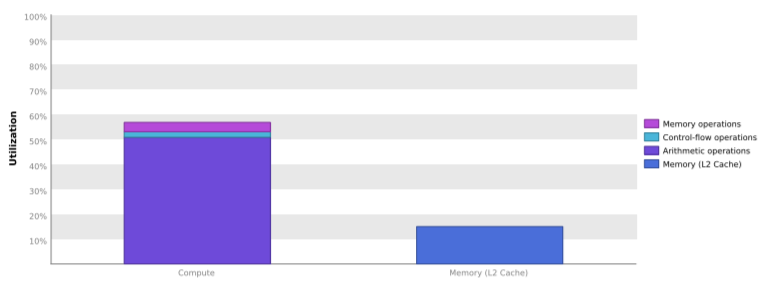
\includegraphics{contents/pics_1/nvvp_gpu.PNG}
    \caption{Kernel performance of \texttt{gpu2}.}
    \label{fig:nvvp_gpu}
\end{figure}

\noindent From figure \ref{fig:nvvp_gpu} above it is evident that too much time is spend on memory. This is quite surprising since matrix-matrix multiplication should be compute-bound for large problem sizes and not memory-bound. The \texttt{nvvp} profiler reveals that only 20 registers are used, while others (e.g. Hans Henrik) were able to use 32 registers. This automatically results in too many cache-misses since the 20 registers cannot store as much information, and hence memory has to be fetched more often. Therefore, time that could be spend on computing is instead spend on waiting for the memory to be loaded.\\

\noindent Unfortunately it was not clear what caused this low number of registers and how it could be increased, and therefore the issue could not be solved in time.\\

\noindent Similar problems occurred for the other versions: for \texttt{gpu3} the number of registers is 24, for \texttt{gpu4} the number is 27, and for \texttt{gpu5} the number of registers is 32. Even though the number of registers increased for each version, too much time was still spend on memory. It is possible that the new driver (which was not used due to time issues) would solve this problem. Another idea would be to run the driver on a different node.\\

\noindent A second suggestion for further improving the kernels applies to all of the different versions. Every single time an element of $A$ is multiplied by an element of $B$, global memory is accessed (by updating the corresponding element of $C$) which is very time consuming. This could be solved by using a local variable inside the kernel instead. I.e. if a local variable \texttt{C\_value} was used to store the intermediate value of the current element of $C$, it would only be necessary to access global memory once for each element of $C$ instead of every time an element of $A$ is multiplied by an element of $B$.\\

\noindent The implementation of version 5 actually uses a local variable inside the kernel, and this probably explains some of the extra speed-up compared to the other versions.

\newpage
\section{Poisson problem}
This section includes several algorithms/kernels, results and analysis of those performances. 
The performance of the kernel setups will be compared and they have been evaluated for $N = 2048$ and \texttt{max\_iter} = $1000$. The chosen parameters gives the refrence algorithm a runtime of $\approx1.5$ secound.

\noindent The main purpose of this section is to find the speedup for difference GPU implementations in reference of the best OpenMP (\texttt{jac\_cpu}) version from previous assignment. The environment variable which determines the wait policy of the threads has not been set to \texttt{OMP\_WAIT\_POLICY=active} is in the previous assignment. The OpenMP is evaluated with \texttt{OMP\_NUM\_THREADS=12}.
The achieved speedups are presented in table \ref{tab:speedup_pos}.

\noindent It has been chosen to validate the implementation of the difference GPU kernels by visualizing their estimates of $u(x,y)$ after the last iteration. This give a visual verfication of the kernel and source implementations. See plots in figure \ref{fig:apped_vis_pos} in the appendix.

\noindent The iterative process is controlled by the host and it uses \texttt{cudaDeviceSynchronize()} to make sure the work of the threads on the devices is done before incrementing the iteration. The iterative process \texttt{while(k < max\_iter)} which includes pointer switchs and new kernel calls is identical for all three GPU versions. Although the kernels are called by different 
kernel launch parameters: \texttt{<<<grid,block>>>}.

\noindent The initialization of the boundary conditions in $u$ and $u\_old$, and of the heating source given by $f$ are done on the on the host. The and copied to the device by using the approiate cuda calls.  
The I/O duration for transferring the initial matrices to the device and the duration of the transferring the estimate of $u$ back to host is included in the total compute time in order to make a fair comparison to the \texttt{jac\_cpu} function.



\subsection{Sequential GPU Jacobi}
The kernel used in the Sequential Poisson is provided in algorithm \ref{alg:jac_v1}. 

\noindent \texttt{jac\_gpu1} is called by the following launch parameters \texttt{<<<1,1>>>jac\_gpu1}. This ensures it only enables one block with one thread. See algo. \ref{alg:app_jac_v1} for the complete source code.

\lstinputlisting[label={alg:jac_v1},caption={Algo. \texttt{jac\_gpu1}.},style=CStyle, linerange={23-33}]{code_3/jac_gpu1.cu}.

\subsection{Naive GPU Jacobi}
The Naive Poisson kernel have been implemented by using one thread per grid point which enables the high parallelism of the device. The implementation uses global memory and line 2-3 shows how the upadted element is determined. The kernel is presented in algo. \ref{alg:jac_v2}.

\lstinputlisting[label={alg:jac_v2},caption={Algo. \texttt{jac\_gpu2}.},style=CStyle, linerange={24-31}]{code_3/jac_gpu2.cu}. 


\noindent The kernel is called by following launch paramters: \texttt{<<<dim\_grid,dim\_block>>>jac\_gpu2} which creates a 2D thread blocks. The 2D grid and block size are given by:
\begin{align}
dim3 \quad &dim\_grid \left(  \frac { N+bs-1 }{ bs },\frac { N+bs-1 }{ bs } \right)  \\
dim3\quad  &dim\_block\left(bs, bs \right)
\end{align}
where $bs=16$ is the number of threads in each block.


\subsubsection{\texttt{nvvp}}
The \texttt{nvvp} analyzing tool tells that the \texttt{jac\_gpu2()} has a "Low Compute Utilization" $\approx 16\%$, presented in figure \ref{fig:computebound}. This is as expected, as all memory is fetched globally in the implementation, and as only few floating point operations are performed every time memory is retrieved. Due to this difficulty, the Jacobi method is memory bound. This could be optimized by splitting up the copying, such that the algorithm could copy and compute simultaneously and hereby reduce the computation time. By using more specialized analysis tools within \texttt{nvvp}, a bandwidth limitation is proposed. This limits also supports the claim that the problem is memory bound.  The solution to the Poisson problem using this algorithm is presented in \ref{fig:jac_gpu2} in the appendix.\\

\begin{figure}[H]
\centering
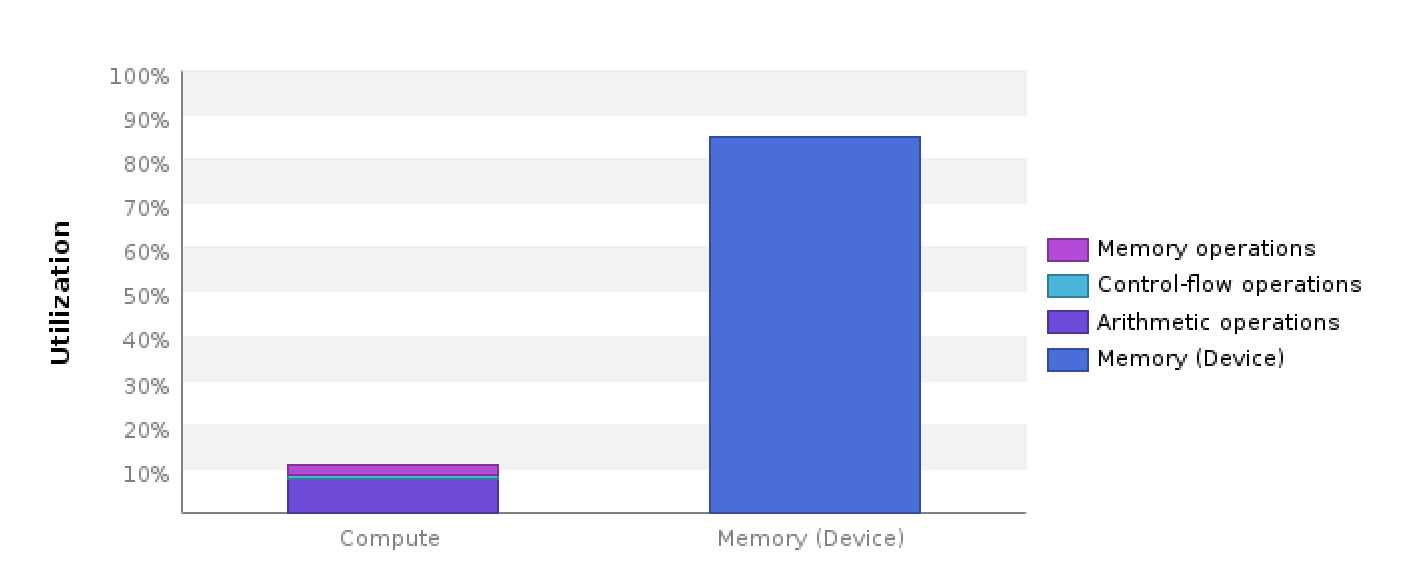
\includegraphics[width=1\textwidth]{data_3/pos_sceenshots/computebound.png}
\caption{The \texttt{nvvp} analysis of \texttt{jac\_gpu2()}. This reports that the algorithm is memory bound as the percentage of utilized memory is much bigger than the utilization of the computation.}
\label{fig:computebound}
\end{figure}

%Vi bruger lang tid på at copiere data, dette kunne blive forbredet hvis man kun kopierede lidt over af gangen . low compute utilization (16\%) pga lang tid om at kopiere. N = 2048, 1000 iterationer. low kernel concurrency.  



\subsection{Multiple GPU Jacobi}
The third version the Jacobi version use multiply (two) GPUs. The problem is hereby split equally between the devices. It has been chosen to create a horizontal split.

\noindent The kernels, \texttt{jac\_gpu3}, used to solve the Poisson problem is presented in algorithm \ref{alg:jac_v3_alg}. 

\noindent The \texttt{cudaDeviceEnablePeerAccess()} method is used to solve the boarder issues between the top and bottom problem as the Jacobi iteration uses the adjacent grid points when updating an element. See the complete source implementation, algo. \ref{alg:app_jac_v3} in the appendix.

\lstinputlisting[label={alg:jac_v3_alg},caption={Algo. \texttt{jac\_gpu3}.},style=CStyle, linerange={26-46}]{code_3/jac_gpu3.cu}

\noindent The kernel is, as in \texttt{jac\_gpu2}, called by the following launch paramters: \texttt{<<<dim\_grid,dim\_block>>> jac\_gpu3}. Noticeable the grid is $N/2$ in the second axis in order to support the dimensions of the each subproblem. The 2D grid and block size are given by:
\begin{align}
dim3 \quad &dim\_grid \left(  \frac { N+bs-1 }{ bs },\frac { N/2+bs-1 }{ bs } \right)  \\
dim3\quad  &dim\_block\left(bs, bs \right)
\end{align}



\subsection{Speedup}
The expected compute speedup is 8x\footnote{PerformanceTuningIntro.pdf, slide 20.} when deploying the algorithm on the GPU compared to the CPU.
Table \ref{tab:speedup_pos} reports the achieved speedups for the three implementations.

\begin{table}[!th]
\centering
\begin{tabular}{l|r}
Algo. & Speedup \\\hline
\texttt{cpu}&1.0000x \\
\texttt{gpu1}&0.0021x \\
\texttt{gpu2}&10.3818x \\
\texttt{gpu3}&16.5419x \\

\end{tabular}
\caption{This table present the speed-ups of \texttt{jac\_gpu1}, \texttt{jac\_gpu2} and, \texttt{jac\_gpu3} in reference to the fastest CPU version from assignment 2, \texttt{cpu()} }
\label{tab:speedup_pos}
\end{table}

\noindent As expected the \texttt{jac\_gpu1} does not gain any improvements. The reason why is the lack of parallelism. Hence there is only launched one block with one kernel.

\noindent The speedup gained by \texttt{jac\_gpu2} is $\approx 10x$ which slightly higher than the expected compute speedup. This can be caused by a version of the OpenMP implementation, which is not fully optimized. If the implementation is sub-optimal the comparison is not fair to the fully parallel implementation on the GPU.

\noindent When splitting the problem into two subproblems the expected speedup is \underline{not} $2x$ between \texttt{jac\_gpu2} and \texttt{jac\_gpu3}. The reason is due to the nature of the Jacobi algorithm. There needs to be shared global memory access between the two devices in order to update the "middle" horizontal boarders elements. The shared global memory, accessed by peer access, is transferred on the PCIe express bus which introduce a latency and therefore not able to scale $2x$. 

% \begin{figure}[H]
% \centering
% \begin{tikzpicture}[scale = 1]
% \begin{axis}[
%     width=10cm, height=8cm,     % size of the image
%     ybar,
%     %symbolic x coords={},
%     xticklabels={\texttt{jac\_cpu},\texttt{jac\_gpu1},\texttt{jac\_gpu2},\texttt{jac\_gpu3}},
%     xtick=data,
%     ytick={0,1,2,9,10,11,15,16,17},
%     ylabel=x,
%     %xlabel=Algo,
%     ]
    
% \addplot table [x=x, y=speed, col sep=comma]{data_3/performance_pos.txt};
    
% %\addplot table[x=interval,y=carT]{\mydata};
% \end{axis}
% \end{tikzpicture}
% \caption{Caption}
% \label{fig:speedup_pos}
% \end{figure}





\newpage
\section{Conclusion}
In the part concerning matrix-matrix multiplication, the analysis shows that there is a significant performance gain in using GPUs. used in \texttt{lib} to four. It is especially seen how shared memory improves the performance by considering \texttt{gpu2} and \texttt{gpu5}. Both algorithms uses one thread pr element in $C$, but the performance of \texttt{gpu5} is much higher, as the algorithm takes advantage of shared memory. The measured speed-ups might be overestimated due to using a driver, that limits the number of threads. If the updated driver had been used, the performance of \texttt{lib} might have been much better. Regarding the implementation of the algorithms, the \texttt{nvvp} profiler analysis showed that relatively few registers are used pr. thread. This limits the performance, as a lot of time is used on copying memory back and forth. This alone was not enough to explain the amount of time used on memory on the device, why it was discovered that every time an addition was made to an element in $C$, this was stored and fetched from the global memory. The kernels could have been optimized by saving the element of $C$ locally while computing it and then writing it to the global variable \texttt{d\_C}. \\
The experimentally achieved speed-ups reported table \ref{tab:speedup_pos} indicates a very good reason for performing this scientific computing problem on a many core multiprocessor such as a GPU or multiply GPUs compared to a traditional multi core CPU using a single treads pr. core.
The enhancement by performing the Jacobi algorithm on the GPU is $\approx 10x$. Splitting the problem into two subproblems scales further to $\approx 16x$.
\printbibliography
\newpage
\begin{appendices}
\section*{Algo. \texttt{jac\_mp\_v23()}}
The change between version 2 and version 3 is in its corresponding main files, see file \texttt{main\_jac\_mp\_v2.c} and file \texttt{main\_jac\_mp\_v3.c}.

\lstinputlisting[label={alg:app_jac_mp_v23},caption={Algo. \texttt{jac\_mp\_v2()} and \texttt{jac\_mp\_v3()}.},style=CStyle, linerange={169-206}]{code_2/func.c}

\newpage
\section*{Algo. \texttt{mandel()}}
\lstinputlisting[label={alg:app_mandel},caption={Algo. \texttt{mandel()}.},style=CStyle, linerange={248-291}]{code_2/func.c}

\section{\texttt{lib}}
\lstinputlisting[label={alg:CPU_lib},caption={Implementation of the library function \texttt{cblas\_dgemm}},style=CStyle, linerange={303-313}]{code_3/func_cu.tex}


\newpage
\section{\texttt{jac\_cpu()}}
\lstinputlisting[label={alg:app_jac_v0},caption={Algo. \texttt{jac\_cpu()}.},style=CStyle]{code_3/jac_cpu.c}


\newpage
\section{\texttt{jac\_gpu1()}}
\lstinputlisting[label={alg:app_jac_v1},caption={Algo. \texttt{jac\_gpu1()}.},style=CStyle]{code_3/jac_gpu1.cu}

\newpage
\section{\texttt{jac\_gpu2()}}
\lstinputlisting[label={alg:app_jac_v2},caption={Algo. \texttt{jac\_gpu2()}.},style=CStyle]{code_3/jac_gpu2.cu}


\newpage
\section{\texttt{jac\_gpu3()}}
\lstinputlisting[label={alg:app_jac_v3},caption={Algo. \texttt{jac\_gpu3()}.},style=CStyle]{code_3/jac_gpu3.cu}




\newpage
\section{Visual Estimates of $u(x,y)$}

The following plots in figure \ref{fig:apped_vis_pos} visualizes the estimates of $u(x,y)$ for the four given approaches, \texttt{jac\_cpu}, \texttt{jac\_gpu1}, \texttt{jac\_gpu2} and \texttt{jac\_gpu3}.
The algorithms have been running for $1000$ iterations and for $N=2048$.

\begin{figure}[!th]
\centering
\begin{subfigure}{.5\textwidth}
  \centering
  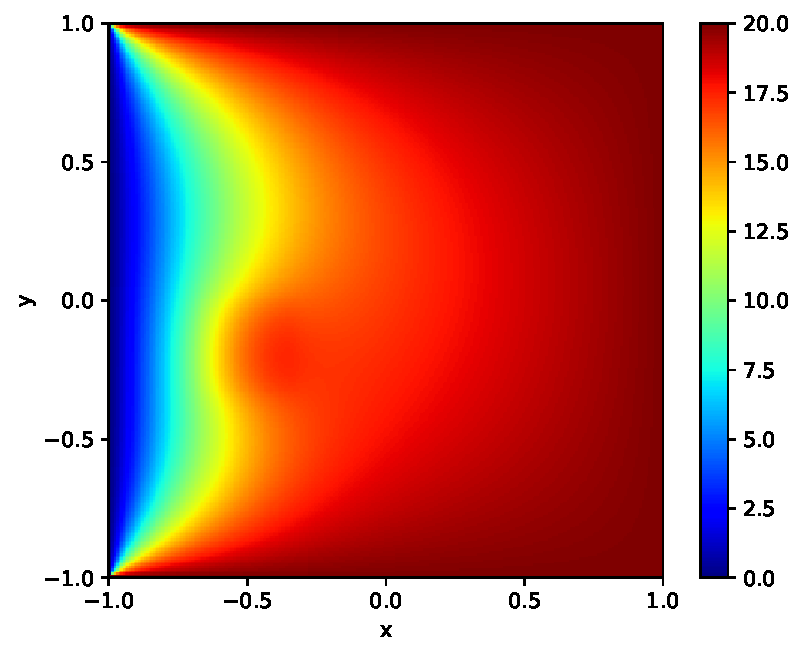
\includegraphics[width=.9\linewidth]{data_3/pos/jac_cpu.pdf}
  \caption{\texttt{jac\_cpu}}
  \label{fig:jac_gpu}
\end{subfigure}%
\begin{subfigure}{.5\textwidth}
  \centering
  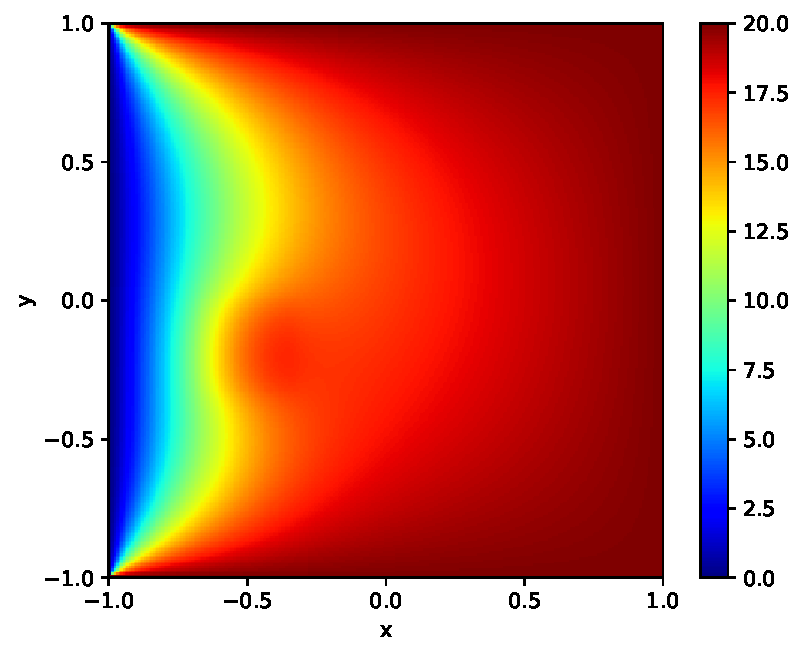
\includegraphics[width=.9\linewidth]{data_3/pos/jac_gpu1.pdf}
  \caption{\texttt{jac\_gpu1}}
  \label{fig:jac_gpu1}
\end{subfigure}
\begin{subfigure}{.5\textwidth}
  \centering
  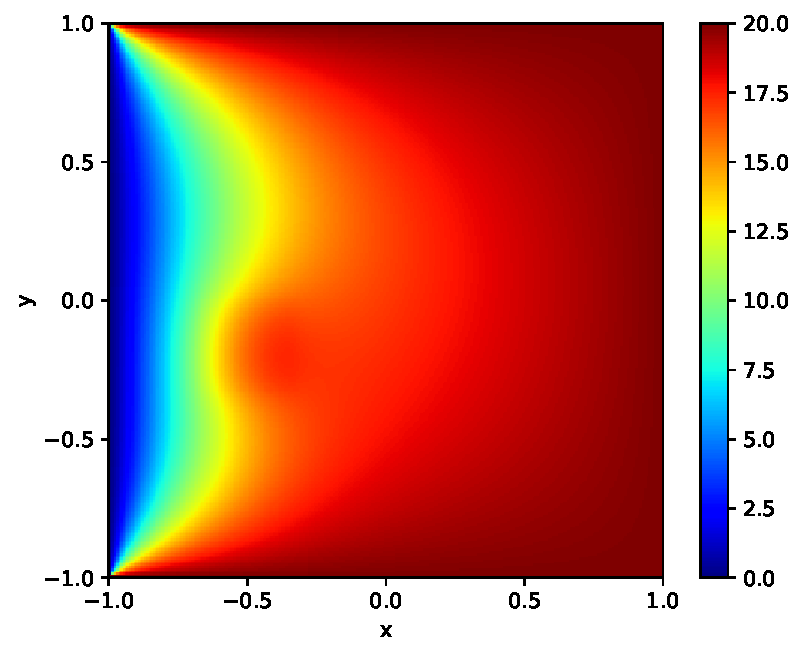
\includegraphics[width=.9\linewidth]{data_3/pos/jac_gpu2.pdf}
  \caption{\texttt{jac\_gpu2}}
  \label{fig:jac_gpu2}
\end{subfigure}%
\begin{subfigure}{.5\textwidth}
  \centering
  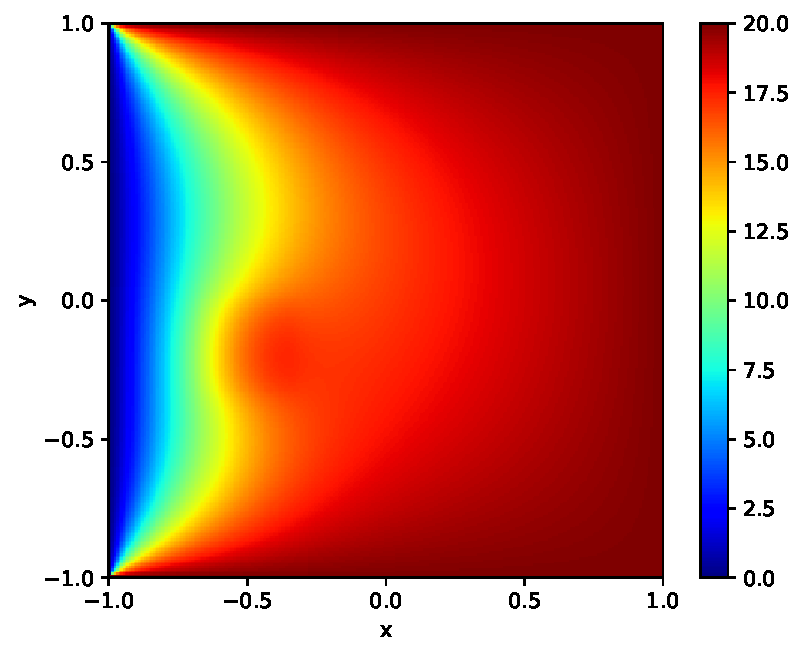
\includegraphics[width=.9\linewidth]{data_3/pos/jac_gpu3.pdf}
  \caption{\texttt{jac\_gpu3}}
  \label{fig:jac_gpu3}
\end{subfigure}
\caption{Estimate of the function $u(x,y)$.}
\label{fig:apped_vis_pos}
\end{figure}
\end{appendices}
\end{document}